\RequirePackage{fix-cm}
\documentclass[12pt,letterpaper]{article}
\usepackage[margin=1in,headheight=15pt,headsep=15pt]{geometry}
\usepackage{amsmath,amssymb,graphicx,booktabs,array,float,fancyhdr,lastpage,hyperref,listings,xcolor}
\usepackage{microtype,needspace,fontspec}
\usepackage[UTF8,fontset=none,scheme=plain]{ctex}
\usepackage{capt-of}
\usepackage{tikz}
\usetikzlibrary{arrows.meta}
\setmainfont{Times New Roman}
\setCJKmainfont{SimSun}[BoldFont=SimHei,ItalicFont=KaiTi,BoldItalicFont=KaiTi]
\setCJKsansfont{SimHei}
\setCJKmonofont{SimSun}[BoldFont=SimHei,ItalicFont=KaiTi]
\ctexset{contentsname=目录,figurename=图,tablename=表}
\renewcommand{\refname}{参考文献}
\setlength{\emergencystretch}{3em}
\setlength{\parindent}{2em}
\hypersetup{colorlinks=false,hidelinks}
\pagestyle{fancy}\fancyhf{}
\fancyhead[L]{\normalsize 题目 B}
\fancyhead[C]{\small 国际大学生物理竞赛}
\fancyhead[R]{\small 第 \thepage\ 页，共 \pageref{LastPage} 页}
\renewcommand{\headrulewidth}{0.4pt}
\setlength{\parindent}{2em}
\setlength{\parskip}{0pt}
\lstset{basicstyle=\ttfamily\footnotesize,breaklines=true,numbers=left,numberstyle=\tiny,numbersep=8pt,columns=fullflexible,showstringspaces=false,frame=none}
\graphicspath{{../results/structure_linear_spin/figures/}{aerodynamics/}{assets/}{figures/}}
% Generated from results/structure_v2; do not edit numerical values manually.
\newcommand{\ProblemY}{2.683}
\newcommand{\ProblemZ}{1.959}
\newcommand{\ProblemTime}{0.4026}
\newcommand{\ProblemAlphaD}{1.0001}
\newcommand{\ProblemAlphaL}{1.0000}
\newcommand{\ProblemSpin}{126.51}
\newcommand{\ProblemResidual}{\ensuremath{6.4\times10^{-13}}}
\newcommand{\ProblemSpeedMin}{24.99}
\newcommand{\ProblemSpeedMax}{32.57}
\newcommand{\ProblemReMin}{3.67}
\newcommand{\ProblemReMax}{4.78}
\newcommand{\ProblemSpMin}{0.427}
\newcommand{\ProblemSpMax}{0.557}
\newcommand{\ProblemVX}{30.406}
\newcommand{\ProblemVY}{9.426}
\newcommand{\ProblemVZ}{6.906}
\newcommand{\ProblemWX}{-49.090}
\newcommand{\ProblemWY}{-31.483}
\newcommand{\ProblemWZ}{-112.266}
\newcommand{\ReferenceCD}{0.2415}
\newcommand{\ReferenceCL}{0.2898}
\newcommand{\ForwardInitialTable}{\begin{table}[H]\centering\small
\caption{按正文方法重建的受控正向算例初始条件。}\label{tab:forward-initial}
\begin{tabular}{lrrrrr}\toprule
发射 & $x_0$ (m) & $z_0$ (m) & $v_{x0}$ (m/s) & $v_{z0}$ (m/s) & $\omega_{y0}$ (rad/s)\\\midrule
无旋转 & 0.0001 & 0.8501 & 16.689 & 6.743 & 0.00\\
上旋 a & 0.0001 & 0.8499 & 16.825 & 7.366 & 82.57\\
上旋 b & 0.0001 & 0.8499 & 18.194 & 6.810 & 44.56\\
上旋 c & -0.0070 & 0.8526 & 17.383 & 8.188 & 125.16\\
上旋 d & -0.0067 & 0.8500 & 18.770 & 10.863 & 47.75\\
\bottomrule\end{tabular}\end{table}
}
\newcommand{\ForwardMFourRange}{21.871}
\newcommand{\ForwardMFourError}{-0.029}
\newcommand{\ForwardRangeTable}{\begin{table}[H]\centering\small
\caption{无旋转受控发射的预测射程与带符号误差；文献实测射程为 21.9 m。}\label{tab:forward-range}
\begin{tabular}{lrr}\toprule
模型 & 射程（m） & 预测减去实测（m）\\\midrule
M1 & 24.650 & +2.750\\
M2 & 20.656 & -1.244\\
M3 & 20.656 & -1.244\\
M4 & 21.871 & -0.029\\
\bottomrule\end{tabular}\end{table}
}
\newcommand{\ForwardSpinTable}{\begin{table}[H]\centering\small
\caption{四组上旋片段在实测水平位置处的高度均方根误差（m）。}\label{tab:forward-spin}
\begin{tabular}{lrrrr}\toprule
发射 & M1 & M2 & M3 & M4\\\midrule
a & 0.0119 & 0.0118 & 0.0062 & 0.0072\\
b & 0.0396 & 0.0397 & 0.0459 & 0.0466\\
c & 0.0100 & 0.0100 & 0.0047 & 0.0099\\
d & 0.0171 & 0.0170 & 0.0090 & 0.0082\\
\bottomrule\end{tabular}\end{table}
}
\newcommand{\ProblemResultsTable}{\begin{table}[H]\centering\small
\caption{题目给定观测的逆向预测；残差为早期坐标最大绝对差。}\label{tab:problem}
\begin{tabular}{lrrrrrr}\toprule
模型 & $\alpha_D$ & $\alpha_L$ & 残差（m） & $y_g$ (m) & $z_g$ (m) & $t_g$ (s)\\\midrule
M1 & --- & --- & 0.016 & 3.217 & 1.957 & 0.3706\\
M2 & 1.5683 & --- & 0.01 & 3.217 & 1.879 & 0.4058\\
M3 & 1.5666 & 1.0000 & \ensuremath{1.5\times10^{-12}} & 2.661 & 1.938 & 0.4008\\
M4 & 1.0001 & 1.0000 & \ensuremath{6.4\times10^{-13}} & 2.683 & 1.959 & 0.4026\\
\bottomrule\end{tabular}\end{table}
}
\newcommand{\MatchResultsTable}{\begin{table}[H]\centering\small
\caption{五组实测飞行与四类逆向模型的完整结果；误差为球门平面 $(y,z)$ 的欧氏距离。}\label{tab:match-results}
\begin{tabular}{lllrr}\toprule
事件 & 模型 & 终止状态 & 早期残差（m） & 交点误差（m）\\\midrule
WOH 0487 （头球） & M1 & 到达平面 & 0.036 & 0.717\\
WOH 0487 （头球） & M2 & 到达平面 & 0.00501 & 2.348\\
WOH 0487 （头球） & M3 & 到达平面 & \ensuremath{2.28\times10^{-12}} & 1.909\\
WOH 0487 （头球） & M4 & 触地 & \ensuremath{3.53\times10^{-10}} & ---\\
WOH 0606 （脚部） & M1 & 到达平面 & 0.0263 & 4.988\\
WOH 0606 （脚部） & M2 & 触地 & 0.0303 & ---\\
WOH 0606 （脚部） & M3 & 触地 & \ensuremath{1.32\times10^{-12}} & ---\\
WOH 0606 （脚部） & M4 & 触地 & \ensuremath{1.83\times10^{-10}} & ---\\
WOH 0968 （脚部） & M1 & 触地 & 0.124 & ---\\
WOH 0968 （脚部） & M2 & 触地 & 0.124 & ---\\
WOH 0968 （脚部） & M3 & 提前终止 & 0.127 & ---\\
WOH 0968 （脚部） & M4 & 到达平面 & 0.126 & 10.893\\
WQQ 1227 （头球） & M1 & 到达平面 & 0.18 & 2.785\\
WQQ 1227 （头球） & M2 & 到达平面 & 0.172 & 3.325\\
WQQ 1227 （头球） & M3 & 拟合失败 & 0.0226 & ---\\
WQQ 1227 （头球） & M4 & 拟合失败 & 0.0952 & ---\\
点球 & M1 & 到达平面 & 0.204 & 0.853\\
点球 & M2 & 到达平面 & 0.204 & 0.853\\
点球 & M3 & 拟合失败 & 0.208 & ---\\
点球 & M4 & 拟合失败 & 0.208 & ---\\
\bottomrule\end{tabular}\end{table}
}
\newcommand{\MatchAggregateTable}{\begin{table}[H]\centering\small
\caption{到达球门平面算例的误差与各终止状态计数，逐事件误差见前表。}\label{tab:match-aggregate}
\begin{tabular}{lrrrrr}\toprule
模型 & 到达 & 触地 & 其他 & 拟合失败 & 平均误差（m）\\\midrule
M1 & 4/5 & 1 & 0 & 0 & 2.336\\
M2 & 3/5 & 2 & 0 & 0 & 2.175\\
M3 & 1/5 & 1 & 1 & 2 & 1.909\\
M4 & 1/5 & 2 & 0 & 2 & 10.893\\
\bottomrule\end{tabular}\end{table}
}
\newcommand{\MatchDiscussion}{M1 在五组飞行中有四组到达球门平面，M2 为三组，M3、M4 各为一组。M1 在这些记录中给出最多的球门交点预测。表中同时报告到达算例的平均误差与对应数量。较大的气动力修正及迭代上限情况表明，预测对早期记录运动十分敏感。拟合失败表示达到数值迭代上限，相应候选轨迹保存在计算记录中。}
\newcommand{\TorqueViscousRatio}{\ensuremath{9.8\times10^{-5}}}
\newcommand{\TorqueDisplacement}{0.147}
\newcommand{\TorqueResults}{加入阻尼后，球门交点为 $(2.541,1.996)$ m，恒定自旋时为 $(2.683,1.959)$ m。交点位移为 0.147 m，占 11 m 飞行距离的 1.34\%；自旋减小 41.24\%，到达球门的时间变化为 $-1.60$\%。再加入较弱的黏性项后，阻尼交点变化为 $6.5\times10^{-6}$ m。因此，该参考力矩明显改变自旋，同时使短程飞行终点发生较小而可量化的变化。}
\newcommand{\WindResultsTable}{\begin{table}[H]\centering\small
\caption{反演初速度下的示例风速估算；百分比表示气动系数固定时的动压变化。}\label{tab:wind}
\begin{tabular}{rrrrr}\toprule
$w$ (m/s) & 逆风（\%） & 顺风（\%） & 横风（\%） & 来流夹角（$^\circ$）\\\midrule
1 & +6.23 & -6.05 & +0.09 & 1.76\\
3 & +19.27 & -17.57 & +0.85 & 5.26\\
5 & +33.06 & -28.34 & +2.36 & 8.73\\
\bottomrule\end{tabular}\end{table}
}
\newcommand{\WindThreshold}{0.80}


\begin{document}
\begin{center}
{\Large\bfseries 足球三维飞行至球门的建模与实测对照\par}
\vspace{2mm}{\bfseries 题目 B\par}
\vspace{3mm}{\bfseries 摘要\par}
\end{center}
本研究比较仅受重力、加入阻力、恒力和包含马格努斯力四种模型。M3 根据三个位置求取恒加速度；M4 采用恒定阻力系数和与自旋参数成正比的升力系数，反演初速度与气动参数。五组比赛飞行用于对照；题目算例的 M4 球门平面交点为 $(y,z)=(\ProblemY,\ProblemZ)$ m。



\noindent\textbf{关键词：}足球；空气阻力；马格努斯效应；逆向预测；轨迹对照
\newpage\tableofcontents\newpage
\section{引言}
\subsection{问题背景}
点球是一个受到严格时空条件约束的拦截问题。守门员需要在合适的时间到达合适的位置，同时决定何时以及向哪个方向移动。点球预判研究讨论了这一时机问题，并表明射门速度和踢球技术会影响射门方向的可预测性\cite{kamp2018,hunter2018}。这些研究也考虑球员触球前的动作线索；本题则关注足球离脚后，根据已测位置预测其后续位置。

足球踢出后的轨迹通常会发生弯曲。重力使轨迹向下弯曲，空气阻力使足球减速，自旋还会产生侧向或竖直方向的气动力。Bray 和 Kerwin 将空气动力与运动方程结合，并与实际任意球轨迹进行比较\cite{bray}；Myers 和 Mitchell 分析了旋转足球的三维运动及阻力、自旋的影响\cite{myers}；Maponi 和 Piombin 则建立了可考虑风速的数值计算框架\cite{maponi}。

足球表面也会影响气动力。Asai 等通过风洞测量研究了流动条件与足球受力的关系\cite{asai2007}；Paudel 和 Yan 的数值模拟比较了具有真实接缝几何的足球与光滑球体\cite{paudel}。这些研究为先将足球几何形状理想化为球体、再考察气动系数对预测轨迹的影响提供了依据。

真实飞行测量为模型对照提供了基础。Griffiths 等通过球面标记，在场地条件下追踪足球的三维运动与自旋\cite{griffiths2005}。Goff 和 Carr\'e 使用相机记录的飞行轨迹估计气动系数\cite{goff2009}；Goff 等后续结合 29 条飞行轨迹，构建了随速度变化的阻力和升力系数曲线\cite{goff2017}。

本题给出了初始位置及其后的两个早期位置，但没有直接给出初速度、自旋等量。因此，本文利用运动方程寻找与早期观测相符的运动状态，并计算其球门平面交点。DFL 开放数据集同时提供职业比赛事件和光学追踪数据\cite{bassek,dataset}，可用于将预测交点与之后记录的位置进行比较。

\subsection{问题重述}
本文研究足球从点球点附近飞向球门的三维运动。球门宽 7.32 m、高 2.44 m，点球点距球门线 11 m。我们建立包含重力、浮力、阻力与马格努斯效应的模型，求解飞行轨迹及球门平面交点，并与实测点球飞行对照。题目预测使用初始位置及 0.05、0.10 s 的位置，后续位置用于验证。第二章介绍假设与符号，第三章建立受力和运动方程，第四章比较正向与逆向预测，第五章预留灵敏性分析，第六章讨论表面几何、旋转阻尼和风，第七、八章给出小结与模型评价。
\begin{figure}[H]\centering
\resizebox{\textwidth}{!}{% Vector reconstruction of workflow.png: original wording, blocks and connections.
% Use with TikZ and arrows.meta. Coordinates follow the original top-to-bottom layout.
\begingroup
\definecolor{wfInk}{HTML}{263342}
\definecolor{wfBlue}{HTML}{D5EAF8}
\definecolor{wfGreen}{HTML}{D5F0E9}
\definecolor{wfYellow}{HTML}{FFF3CD}
\definecolor{wfWarm}{HTML}{F0DCCB}
\definecolor{wfBorder}{HTML}{81858B}
\begin{tikzpicture}[x=1cm,y=-1cm,
  wfbox/.style={draw=wfInk,line width=1.1pt,rounded corners=9pt},
  wfline/.style={draw=wfInk,line width=1.8pt,line join=round,
    -{Triangle[length=7pt,width=8pt]}},
  wftext/.style={anchor=north west,inner sep=0pt,align=left,
    font=\fontsize{12}{13.5}\selectfont,text=black},
  wftitle/.style={anchor=north,inner sep=0pt,align=center,
    font=\fontsize{15.5}{17.5}\selectfont\bfseries,text=black},
  wfprior/.style={anchor=center,inner sep=0pt,align=center,
    font=\fontsize{12}{13.5}\selectfont,text=black}]


% The arrow network is drawn before the boxes, as in the original figure.
\draw[wfline] (6.43,2.55) -- (6.43,3.66) -- (8.66,3.66) -- (8.66,4.94);
\draw[draw=wfInk,line width=1.6pt] (18.60,1.60) -- (18.60,1.93);
\draw[draw=wfInk,line width=1.6pt] (12.95,1.93) -- (24.25,1.93);
\foreach \px in {12.95,15.82,18.32,21.20,24.25}
  {\draw[wfline] (\px,1.93) -- (\px,2.35);}
\draw[wfline] (18.32,3.85) -- (18.32,4.28) -- (9.70,4.28) -- (9.70,4.94);
\draw[wfline] (14.90,4.28) -- (14.90,4.94);
\draw[wfline] (6.20,7.35) -- (6.85,7.35);
\draw[wfline] (11.70,7.35) -- (12.05,7.35);
\draw[wfline] (19.50,7.35) -- (19.85,7.35);
\draw[wfline] (25.85,7.35) -- (26.20,7.35);
\draw[draw=wfInk,line width=1.8pt] (14.05,9.68) -- (14.05,10.26);
\draw[draw=wfInk,line width=1.8pt] (4.40,10.26) -- (17.95,10.26);
\foreach \px in {4.40,11.45,17.95}
  {\draw[wfline] (\px,10.26) -- (\px,10.85);}
\draw[wfline] (20.55,12.85) -- (21.30,12.85);
\draw[wfline] (26.50,10.85) -- (26.50,9.65);
\draw[wfline] (11.65,15.02) -- (11.65,15.43) -- (24.72,15.43) -- (24.72,14.50);

% Sparse observations and the five prior/bound groups.
\path[wfbox,fill=wfBlue] (2.72,0.61) rectangle (10.17,2.55);
\node[wftitle,font=\fontsize{16.5}{18.5}\selectfont\bfseries] at (6.445,0.95)
  {Sparse Early Observations};
\node[wfprior,font=\fontsize{15.5}{17.5}\selectfont] at (6.445,1.97)
  {$r(0),\ r(0.05\,s),\ r(0.10\,s)$};
\path[wfbox,fill=wfWarm] (12.00,0.55) rectangle (25.20,1.60);
\node[wftitle,font=\fontsize{16.5}{18.5}\selectfont\bfseries] at (18.60,0.83)
  {Physical Inputs \& Model Settings};
\path[wfbox,fill=wfWarm] (11.38,2.35) rectangle (14.52,3.85);
\path[wfbox,fill=wfWarm] (14.72,2.35) rectangle (16.92,3.85);
\path[wfbox,fill=wfWarm] (17.17,2.35) rectangle (19.47,3.85);
\path[wfbox,fill=wfWarm] (19.70,2.35) rectangle (22.70,3.85);
\path[wfbox,fill=wfWarm] (22.92,2.35) rectangle (25.58,3.85);
\node[wfprior] at (12.95,3.10) {Ball geometry \&\\surface model};
\node[wfprior] at (15.82,3.10) {Air density\\\& viscosity};
\node[wfprior] at (18.32,3.10) {Constant\\spin\\reference};
\node[wfprior] at (21.20,3.10) {Still-air\\reference\\setting};
\node[wfprior] at (24.25,3.10) {Published\\$C_D,C_L$\\relations};

% Forces and governing equations.
\path[wfbox,fill=wfGreen] (0.55,4.985) rectangle (6.20,9.715);
\node[wftitle] at (3.375,5.205) {Forces \&\\Governing Equations};
\path[fill=white,fill opacity=.52,rounded corners=9pt]
  (0.73,6.215) rectangle (6.02,9.555);
\node[wftext,text width=5.1cm,font=\fontsize{9.2}{10.5}\selectfont] at (0.92,6.385)
  {\setlength{\jot}{2pt}$\displaystyle\left\{
   \begin{array}{@{}l@{}}
   m\frac{d^2\boldsymbol r}{dt^2}=\boldsymbol F_g+\boldsymbol F_B+\boldsymbol F_D+\boldsymbol F_L\\
   \boldsymbol F_g=-mg\,\boldsymbol e_z\\
   \boldsymbol F_B=\frac43\pi R^3\rho g\,\boldsymbol e_z\\
   \boldsymbol F_D=-qA\alpha_D C_D\frac{\boldsymbol u}{\|\boldsymbol u\|}\\
   \boldsymbol F_L=qA\alpha_L C_L\sin\theta\,\boldsymbol e_L\\
   \dot{\boldsymbol\omega}=\boldsymbol0\\
   q=\rho v^2/2
   \end{array}\right.$};


% State representation, inverse search, integration and goal-plane prediction.
\path[wfbox,fill=wfYellow] (6.85,4.94) rectangle (11.70,9.65);
\node[wftitle] at (9.275,5.15) {State \& Parameter\\Representation};
\node[wftext,text width=4.26cm] at (7.17,6.40)
  {$\bullet$\ Initial motion:\\\hspace*{.32cm}$\boldsymbol v_0,\boldsymbol\omega_0$\\[2pt]
   $\bullet$\ Force corrections:\\\hspace*{.32cm}$\alpha_D,\alpha_L\geq0$\\[2pt]
   $\bullet$\ Forward prediction:\\\hspace*{.32cm}$\alpha_D=\alpha_L=1$.};
\path[wfbox,fill=wfWarm] (12.05,4.94) rectangle (19.50,9.68);
\node[wftitle] at (15.775,5.16) {Inverse Fitting /\\Candidate Parameter Search};
\path[fill=white,fill opacity=.52,rounded corners=9pt]
  (12.28,6.58) rectangle (19.27,9.48);
\node[wftext,font=\fontsize{12}{15}\selectfont] at (12.65,6.90)
  {\begin{tabular}{@{}l@{\hspace{0.16cm}}l@{}}
   $\bullet$ & Fit early positions;\\
   $\bullet$ & Favor corrections close to one;\\
   $\bullet$ & \parbox[t]{5.5cm}{\raggedright Select smallest M4 spin\\among equivalent fits.}
   \end{tabular}};
\path[wfbox,fill=wfBlue] (19.85,4.94) rectangle (25.85,9.65);
\node[wftitle] at (22.85,5.24) {Numerical Integration};
\path[fill=white,fill opacity=.52,rounded corners=9pt]
  (20.04,6.23) rectangle (25.66,9.47);
\node[wftext,font=\fontsize{12.5}{14.5}\selectfont] at (20.28,6.62)
  {\begin{tabular}{@{}l@{\hspace{0.16cm}}l@{}}
   $\bullet$ & Shared force ODE;\\
   $\bullet$ & Constant spin;\\
   $\bullet$ & Update $Re,Sp$;\\
   $\bullet$ & Detect goal-plane crossing.
   \end{tabular}};
\path[wfbox,fill=wfGreen] (26.20,4.94) rectangle (31.40,9.65);
\node[wftitle] at (28.80,5.24) {Goal-Plane\\Prediction};
\path[fill=white,fill opacity=.52,rounded corners=9pt]
  (26.42,6.49) rectangle (31.19,9.48);
\node[wftext,text width=4.50cm,font=\fontsize{12}{13.5}\selectfont] at (26.72,6.70)
  {$\bullet$\ Forward and inverse\\\hspace*{.32cm}crossings $(y,z)$\\[4pt]
   $\bullet$\ Compare trajectory,\\\hspace*{.32cm}range and observed\\\hspace*{.32cm}goal positions.};

% Bottom row: hierarchy, uncertainty, validation, performance.
\path[wfbox,fill=wfBlue] (0.65,10.85) rectangle (7.90,15.15);
\node[wftitle,font=\fontsize{14}{15.5}\selectfont\bfseries] at (4.275,11.05) {Four-Model Hierarchy};
\path[fill=white,fill opacity=.52,rounded corners=9pt]
  (0.85,11.65) rectangle (7.70,14.98);
\node[wftext,text width=6.45cm,font=\fontsize{12}{12}\selectfont] at (1.17,11.78)
  {M1: gravity (baseline)\\[-2pt]
   \hspace*{.14cm}$\downarrow$\\[-2pt]
   M2: gravity and constant drag\\[-2pt]
   \hspace*{.14cm}$\downarrow$\\[-2pt]
   M3: constant drag and Magnus lift\\[-2pt]
   \hspace*{.14cm}$\downarrow$\\[-2pt]
   M4: state-dependent drag and lift};
\path[wfbox,fill=wfWarm] (8.50,10.85) rectangle (14.80,15.02);
\node[wftitle] at (11.65,11.07) {Other Physical\\Factors};
\path[fill=white,fill opacity=.52,rounded corners=9pt]
  (8.73,12.07) rectangle (14.57,14.85);
\node[wftext,text width=5.35cm,font=\fontsize{12}{13.5}\selectfont] at (9.10,12.22)
  {$\bullet$\ surface geometry\\
   $\bullet$\ rotational damping\\
   $\bullet$\ wind-speed estimates\\[4pt]
   Sensitivity analysis is reserved\\for a later section.};
\path[wfbox,fill=wfYellow] (15.30,10.85) rectangle (20.55,14.48);
\node[wftitle] at (17.925,11.08) {Real-Data\\Validation};
\path[fill=white,fill opacity=.52,rounded corners=9pt]
  (15.52,12.17) rectangle (20.33,14.27);
\node[wftext,font=\fontsize{12}{13.5}\selectfont] at (15.78,12.37)
  {\begin{tabular}{@{}l@{\hspace{0.14cm}}l@{}}
   $\bullet$ & \parbox[t]{3.85cm}{\raggedright Use early frames only\\for fitting;}\\[3pt]
   $\bullet$ & \parbox[t]{3.85cm}{\raggedright Reserve future frames\\for testing.}
   \end{tabular}};
\path[wfbox,fill=wfBlue] (21.30,10.85) rectangle (27.53,14.50);
\node[wftitle] at (24.415,11.08) {Performance \&\\Limitations};
\path[fill=white,fill opacity=.52,rounded corners=9pt]
  (21.52,12.17) rectangle (27.31,14.28);
\node[wftext,text width=5.10cm,font=\fontsize{12}{13.5}\selectfont] at (21.94,12.31)
  {$\bullet$\ goal-point error\\
   $\bullet$\ early-position residuals\\
   $\bullet$\ force evolution\\
   $\bullet$\ model comparison};
\end{tikzpicture}
\endgroup
}
\caption{含浮力的受力模型、四类基准模型比较与球门交点预测。}\label{fig:workflow}
\end{figure}


\section{模型准备}
\subsection{基本假设}
\begin{itemize}
\item \textbf{球与脚的作用。} 取足球刚脱离球员脚部、开始自由飞行的时刻为 $t=0$；不对接触期间的冲击过程及球体变形建模。
\item \textbf{刚性球体。} 参照已有足球飞行模型\cite{maponi,bray,myers}，将足球视为质量、半径和迎风面积 $A=\pi R^2$ 恒定的刚性球体，质心与几何中心重合。经验足球气动系数表征表面的平均影响，第~\ref{sec:surface} 节进一步讨论接缝和非对称几何的作用。
\item \textbf{自由飞行。} 自由飞行中考虑重力、空气浮力、空气阻力与自旋升力\cite{maponi,bray}。所研究的飞行在足球首次接触地面、球门结构或其他物体时结束，不考虑碰撞、弹跳和滚动；数值积分在到达指定球门平面时也停止。
\item \textbf{均匀重力场。} 重力加速度为常量，取 $g=9.81\,\mathrm{m/s^2}$。
\item \textbf{大气性质。} 单次飞行中空气密度和动力黏度在空间中保持均匀，气动力通过经验阻力系数和升力系数描述。
\item \textbf{风。} 主计算采用静止空气；考虑风时，单次飞行的风速矢量在空间和时间上保持恒定，忽略小尺度湍流及快速变化的阵风。第~\ref{sec:wind} 节讨论不同风况对相对气流和气动力的影响。
\item \textbf{飞行中的自旋。} 主模型忽略气动力矩，因此自旋向量保持恒定。第~\ref{sec:rotation} 节通过在同一初始状态下加入旋转阻尼，分析这一近似的影响。
\item \textbf{观测与未知参数。} 将题目给出的位置坐标视为准确值。初始位置和随后两个早期位置构成逆向输入，DFL 追踪记录中的后续位置用于比较\cite{bassek,dataset}。在有界不确定性分析中，将无法唯一确定的初速度、自旋、气动参数和环境条件限制在明确的合理范围内；预测不确定性来自这些未确定量和模型假设，而非测量噪声。DFL 记录的竖直坐标按以米为单位的高度处理。
\end{itemize}
\subsection{符号说明}
\begin{table}[H]\centering\small
\caption{主要物理量及题目参考值。}\label{tab:notations}
\begin{tabular}{p{.25\textwidth}p{.46\textwidth}p{.20\textwidth}}\toprule
符号 & 含义 & 数值或单位\\\midrule
$\boldsymbol r,\boldsymbol v$ & 球心位置与速度 & m; m/s\\
$\boldsymbol\omega,\omega$ & 自旋向量及其模长 & rad/s\\
$m,R,A$ & 质量、半径与迎风面积 & 0.43 kg; 0.11 m; $\pi R^2$\\
$g$ & 重力加速度 & 9.81 m/s$^2$\\
$\boldsymbol u,v$ & 相对空气速度及其模长 & m/s\\
$\rho$ & 空气密度 & 1.2 kg/m$^3$\\
$\nu,\mu=\rho\nu$ & 运动黏度与动力黏度 & $1.50\times10^{-5}$ m$^2$/s; Pa\,s\\
$Re,Sp$ & 雷诺数与自旋参数 & 无量纲\\
$C_D,C_L$ & 阻力与横向升力系数 & 无量纲\\
$\alpha_D,\alpha_L$ & 气动力乘法修正系数 & 无量纲\\
$\theta,\boldsymbol e_L$ & 自旋与来流夹角、升力方向 & rad；单位向量\\
$X_g$ & 局部球门平面坐标 & 11 m\\
$\boldsymbol Q,I_b$ & 阻尼力矩与转动惯量（第六章） & N\,m; kg\,m$^2$\\\bottomrule
\end{tabular}\end{table}
题目工况的质量、半径与重力加速度采用 Maponi 和 Piombin 的参考值\cite{maponi}，空气密度取自 Asai 等\cite{asai2007}。运动黏度作为参考空气条件给定，动力黏度按 $\mu=\rho\nu$ 统一计算。受控实验采用各自报告的质量、直径及空气参数。

\section{模型建立}
通过选择纳入的气动力项，同一组牛顿运动方程可形成四类模型。以下先描述几何关系，再将受力与周围流动和球体自旋联系起来。
\subsection{几何与球门平面}
以球场中心为原点、球场长 105 m 时，两条球门线位于 $x=\pm52.50$ m。所选踢球方向朝向正 $x$ 球门。题目局部坐标中，球门开口范围为 $-3.66\le y\le3.66$ m、$0\le z\le2.44$ m。球门交点定义为球心沿前进方向首次到达 $x=X_g$ 时的位置。
\begin{figure}[H]\centering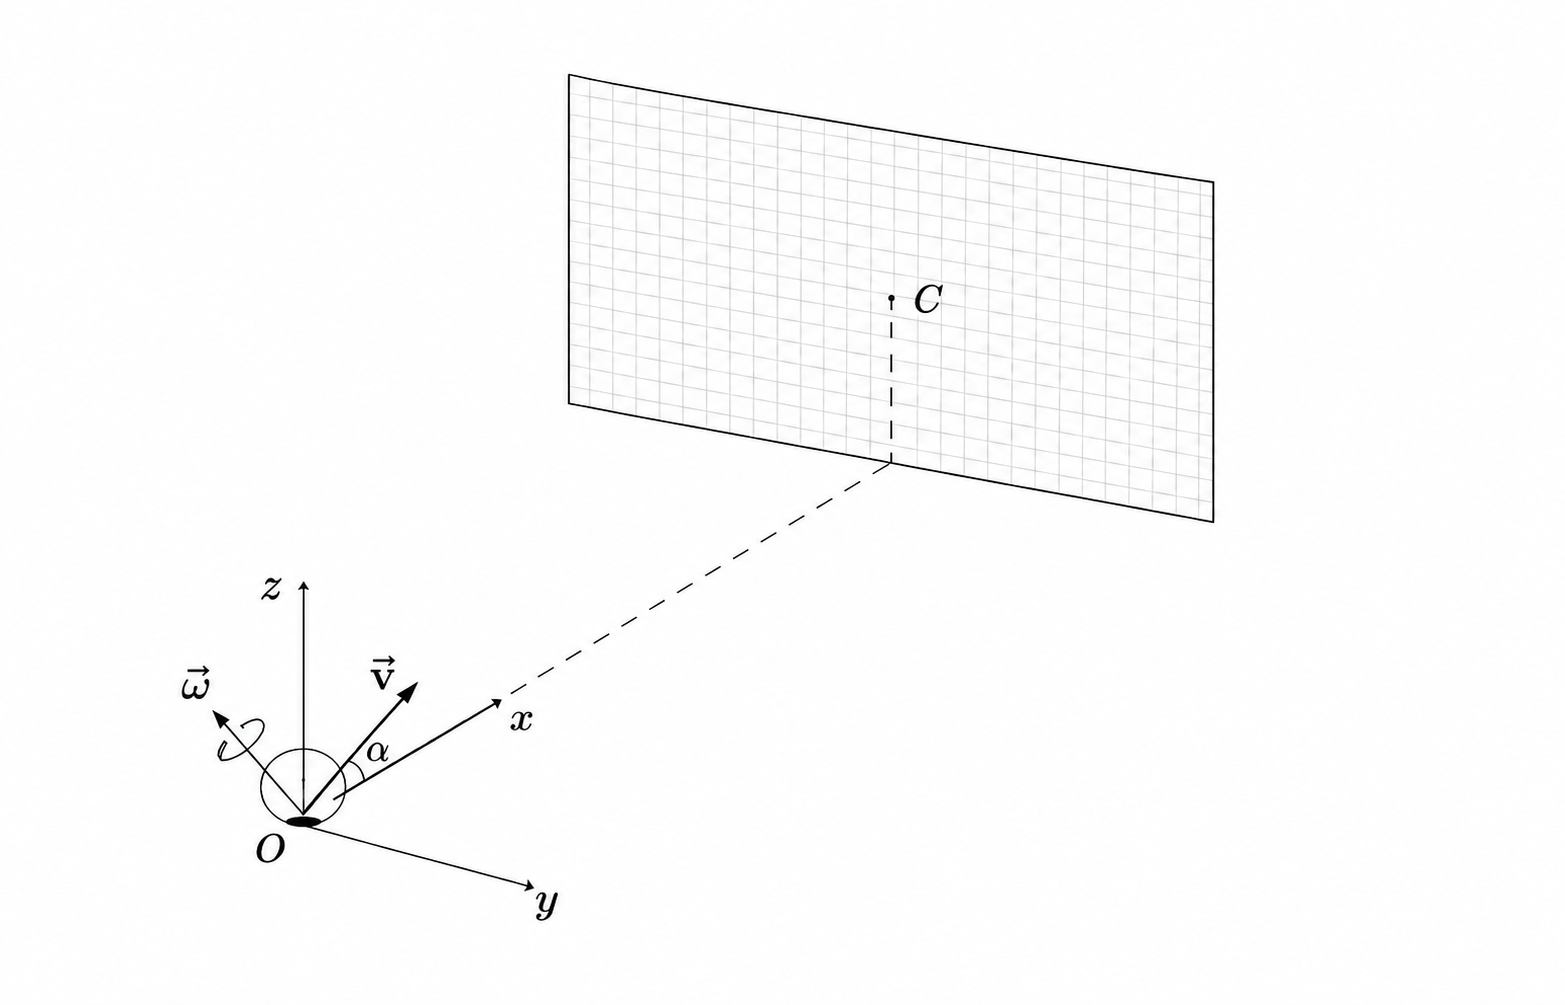
\includegraphics[width=0.78\textwidth]{penalty_geometry_new.png}
\caption{点球局部坐标几何示意。$O$ 为点球点，$C$ 为球门平面上的示意点。}\label{fig:geometry}\end{figure}
题目采用以点球点为原点的局部坐标，球门平面为 $x=11$ m；比赛记录采用球场中心坐标，球门位于 $X_g=52.50$ m。

在 $x=X_g$ 处，若球心满足 $|y|\leq3.66-R$ 和 $R\leq z\leq2.44-R$，足球可完整通过球门开口。球心下降至 $z=R$ 时视为触地。四种模型统一采用上述事件判据。

\subsection{受力分析}
\subsubsection{空气浮力}
依据阿基米德原理，足球排开空气受到的浮力竖直向上。球体积为 $V_b=\frac43\pi R^3$，因而
\begin{equation}
\boldsymbol F_B=\rho V_b g\,\boldsymbol e_z
=\frac43\pi R^3\rho g\,\boldsymbol e_z.
\label{eq:buoyancy}\end{equation}
浮力与重力合并后为 $\boldsymbol F_g+\boldsymbol F_B=-(m-\rho V_b)g\boldsymbol e_z$。对表中参考参数，浮力约为重力的 $1.56\%$，使竖直向下的有效加速度由 $g$ 变为 $g(1-\rho V_b/m)$。

\subsubsection{重力}
重力提供恒定的竖直向下作用力，
\begin{equation}\boldsymbol F_g=-mg\boldsymbol e_z,\end{equation}
其中 $\boldsymbol e_z$ 为竖直向上的单位向量。即使不计气动力，重力也会使轨迹向下弯曲。

\begin{figure}[H]\centering
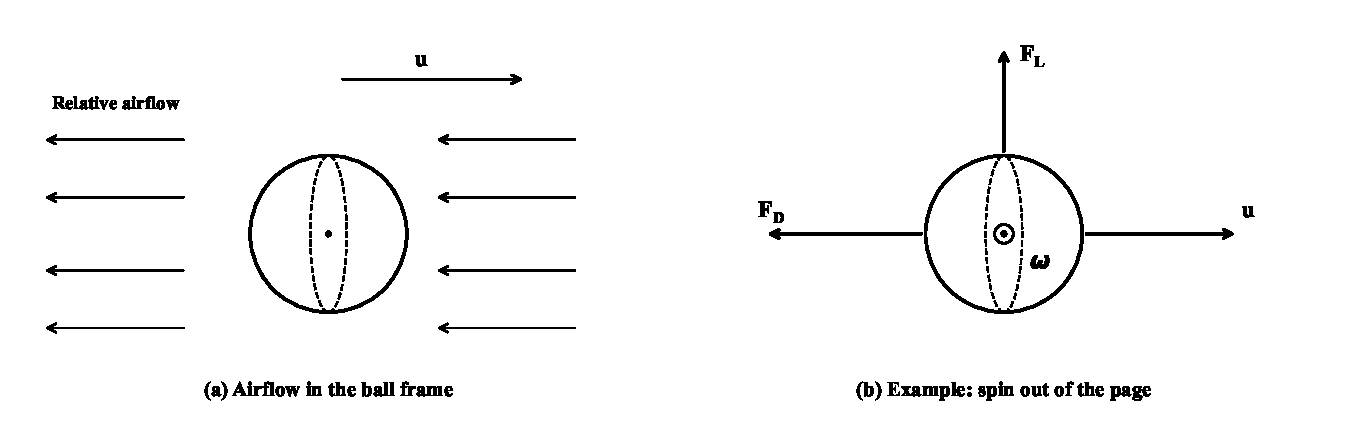
\includegraphics[width=.88\textwidth]{force_schematic.pdf}
\caption{足球周围的相对气流及受力方向示意。$\odot$ 表示自旋轴指向纸面外；左图中的 $\boldsymbol u$ 是足球相对于空气的速度。}\label{fig:force-schematic}\end{figure}

\subsubsection{空气阻力}\label{sec:drag}
足球相对空气的速度为 $\boldsymbol u=\boldsymbol v-\boldsymbol v_{\rm wind}$，令 $u=\|\boldsymbol u\|$、迎风面积 $A=\pi R^2$。阻力与相对速度方向相反，其大小与速度平方成正比\cite{goff2009,kiratidis2018}：
\begin{equation}\boldsymbol F_D=-\tfrac12\rho A C_D u\boldsymbol u.\label{eq:drag-force}\end{equation}
其中 $C_D$ 为无量纲阻力系数，主模型中取常数；静止空气时 $\boldsymbol u=\boldsymbol v$。
\subsubsection{马格努斯升力}\label{sec:lift}
\begin{figure}[H]\centering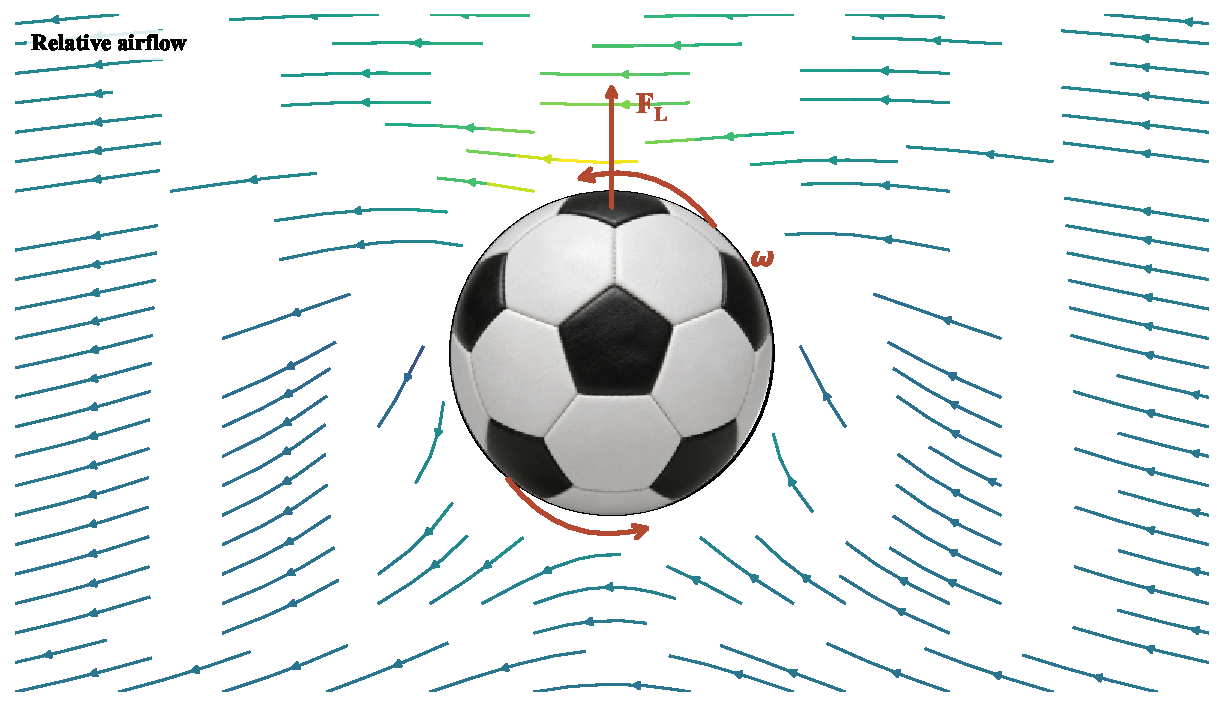
\includegraphics[width=.78\textwidth]{magnus_streamlines.pdf}
\caption{旋转足球周围的理想化相对流线。}\label{fig:magnus-flow}\end{figure}
旋转足球受到垂直于自旋和相对速度的马格努斯力。令 $Sp=R\|\boldsymbol\omega\|/u$，采用简化关系 $C_L=\alpha Sp$，其中 $\alpha$ 为待定常数。代入升力表达式并对斜置旋转轴作投影，得到
\begin{equation}\boldsymbol F_L=\tfrac12\rho A R\alpha(\boldsymbol\omega\times\boldsymbol u).\label{eq:lift-force}\end{equation}
该式在自旋为零或相对速度为零时自然为零。叉乘方向依据本文坐标约定；采用相反的叉乘顺序时须同时调整符号。
\subsection{动力学方程}\label{sec:dynamics}
牛顿第二定律与角动量定律给出
\begin{equation}
m\dot{\boldsymbol v}=\sum\boldsymbol F,\qquad
\frac{d\boldsymbol L}{dt}=\boldsymbol Q,\qquad\boldsymbol L=I_b\boldsymbol\omega.
\end{equation}
外力矩取零、球体转动惯量恒定时，主模型为
\begin{equation}
\left\{\begin{aligned}
\dot{\boldsymbol r}&=\boldsymbol v,\\
m\dot{\boldsymbol v}&=\boldsymbol F_g+\boldsymbol F_B+\boldsymbol F_D+\boldsymbol F_L,\\
\dot{\boldsymbol\omega}&=\boldsymbol0.
\end{aligned}\right.\label{eq:motion}
\end{equation}
相应初始条件为
\begin{equation}
\left\{\begin{aligned}
\boldsymbol r(0)&=\boldsymbol r_0,\\
\boldsymbol v(0)&=(v_{x0},v_{y0},v_{z0}),\\
\boldsymbol\omega(0)&=(\omega_{x0},\omega_{y0},\omega_{z0}).
\end{aligned}\right.\label{eq:initial}
\end{equation}
已知初始位置确定飞行起点，三个初速度分量与三个自旋分量描述初始运动。在静止空气中，阻力消耗机械能，马格努斯力沿速度方向不做功，重力使动能与势能相互转换。

本节给出加入浮力的扩展方程。第~\ref{sec:solving} 节及后续已列数值、图表沿用原有的重力、阻力和马格努斯力计算，即对应 $\boldsymbol F_B=\boldsymbol 0$ 的基准结果；加入浮力后的结果尚未重算。

\section{模型求解}\label{sec:solving}
下面各算例沿用未计浮力的三力基准结果。通过逐步增加气动描述，比较各作用对轨迹的影响。表~\ref{tab:models} 定义四类模型。正向预测采用实测或重建的发射条件，气动力修正系数取一；逆向预测利用两个后续位置反演初始运动与气动力修正，再将该状态推进至球门。
\begin{table}[H]\centering\small
\caption{四类模型与反演量}\label{tab:models}
\begin{tabular}{lll}\toprule
模型 & 运动假设 & 反演量\\\midrule
M1 & 重力 & 初速度 (3)\\
M2 & 重力和阻力 & 初速度、阻力系数 (4)\\
M3 & 恒合力、匀加速度 & 初速度、加速度 (6)\\
M4 & 重力、阻力和马格努斯力 & 初速度、旋转轴、$C_D$、$\alpha$ (7)\\\bottomrule
\end{tabular}\end{table}
M3 的合力包括重力与其他力的合效果。M4 中 $C_D$ 与 $\alpha$ 为常数，$C_L=\alpha Sp$ 随运动变化。正向参考值为 $C_D=\ReferenceCD$、$\alpha=\ReferenceCL$，参考值取自文献参考工况\cite{kiratidis2018}。

\subsection{正向预测}\label{sec:forward}
\subsubsection{求解方法与实验条件}
正向对照使用 M1、M2 和 M4 的给定初始状态与参考气动系数。M3 的恒加速度须由位置反演，故不纳入这些给定初速度的正向对照。

我们选用五组受控飞行：一组无旋转发射，实测射程为 21.9 m；另有四组上旋轨迹。各组初始状态见表~\ref{tab:forward-initial}。

\begin{quote}\small\textbf{数据来源与提取。} Goff 和 Carr\'e\cite{goff2009} 使用质量 0.424 kg、直径 0.218 m 的 32 块面板足球及两台高速相机；报告空气密度为 1.2 kg/m$^3$、运动黏度为 $1.54\times10^{-5}$ m$^2$/s，射程误差不超过 $\pm0.05$ m。我们从其图 3、4、11、14 的矢量 PDF 提取红色实测标记。无旋转案例初速度约 18 m/s、仰角约 $22^\circ$、初始球心高度约 0.85 m，早期标记间隔为 0.005 s；四组旋转案例用已发表的 $Re$、$Sp$ 确定速度与自旋，并以前三个数字化位置确定空间切线，沿 $z(x)$ 比较。\end{quote}

表~\ref{tab:forward-initial} 列出正向输入。各算例位于 $x$--$z$ 平面，$y_0=v_{y0}=0$、$\omega_{x0}=\omega_{z0}=0$，因此表中的 $v_{x0}$、$v_{z0}$、$\omega_{y0}$ 补全了六个初速度和自旋分量。首个标记给出初始位置。
\ForwardInitialTable

\subsubsection{计算轨迹与物理分析}
\ForwardRangeTable
\begin{figure}[H]\centering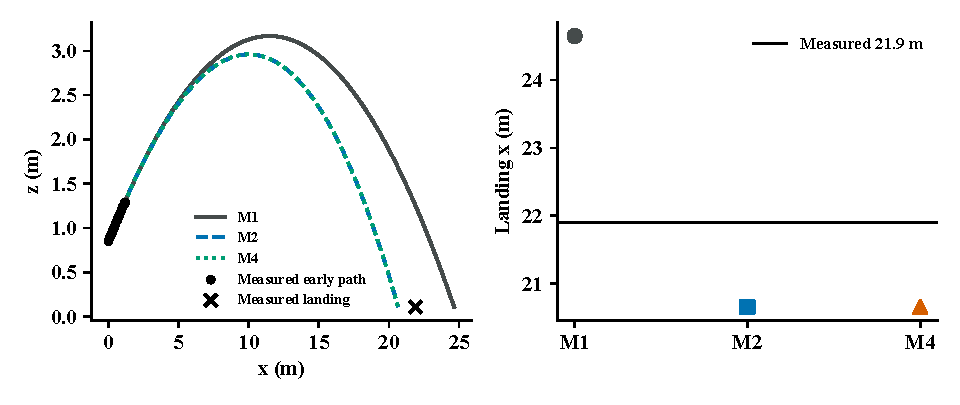
\includegraphics[width=\textwidth]{forward_range.pdf}
\caption{Goff 和 Carr\'e 无旋转实验的正向预测\cite{goff2009}。左图为计算路径、数字化早期位置及实测落点；右图将各模型射程与实测 21.9 m 比较。初始自旋为零时 M2、M4 重合。}\label{fig:forward-range}\end{figure}
仅受重力时射程较远；阻力降低水平速度。无旋转时 M2 和 M4 的参考阻力相同，计算轨迹重合。M4 预测射程与实测之差为 \ForwardMFourError\ m。

\ForwardSpinTable
\begin{figure}[H]\centering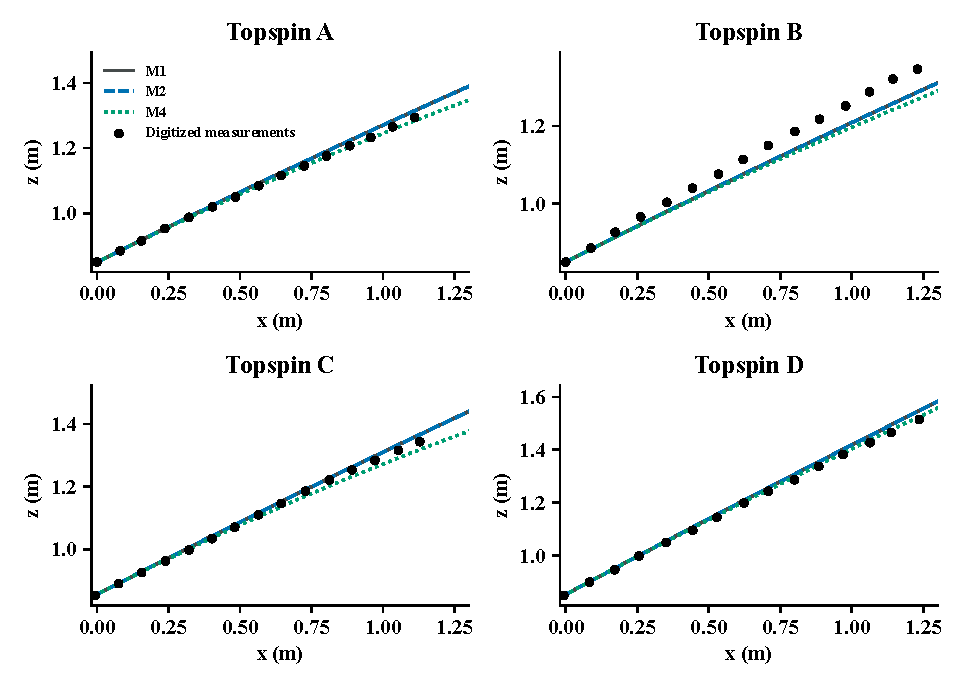
\includegraphics[width=\textwidth]{forward_topspin.pdf}
\caption{从 Goff 和 Carr\'e 原文图 14 提取的四组上旋轨迹\cite{goff2009}。黑点为实测标记中心，各模型采用单位气动力修正和已列初始条件，显示范围为公开的早期空间片段。}\label{fig:forward-spin}\end{figure}
上旋产生向下的马格努斯力。表~\ref{tab:forward-spin} 给出实测水平位置处的高度均方根误差。

\begin{figure}[H]\centering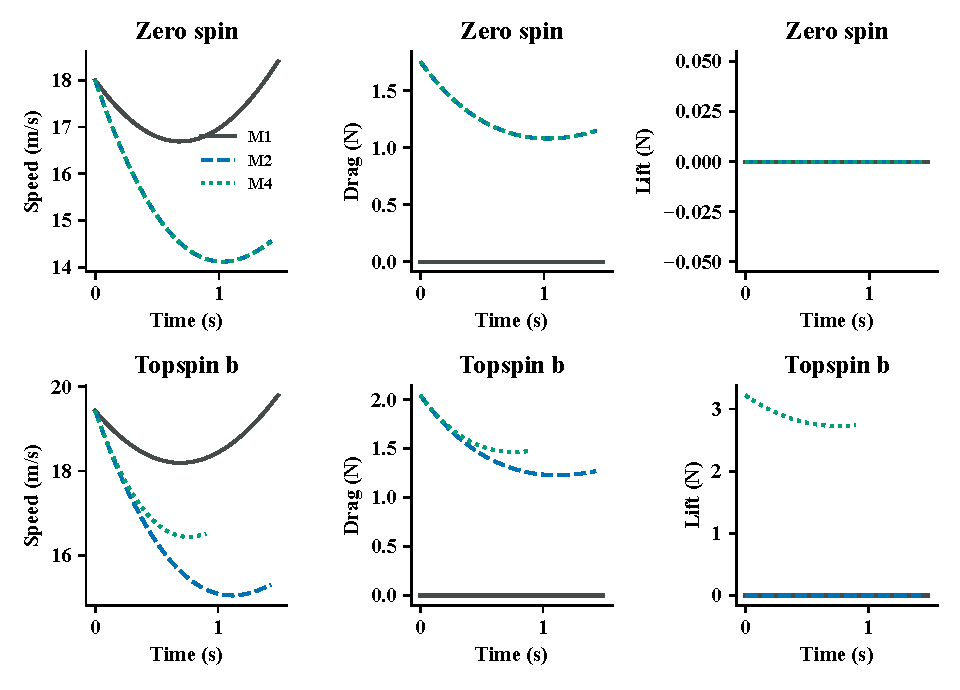
\includegraphics[width=\textwidth]{forward_dynamics.pdf}
\caption{无旋转与上旋 b 正向算例中的速度、阻力和升力。力的大小由同一组方程计算；即使系数恒定，动压随速度变化仍使气动力变化。}\label{fig:forward-dynamics}\end{figure}
球速较高时阻力较强；上旋的向下升力改变竖直运动与飞行时间。固定系数时，气动力大小仍随速度变化。

\subsection{逆向预测}\label{sec:inverse}
\subsubsection{早期位置反演与代表解}
M3 利用三个位置求解恒定加速度：
\begin{equation}\boldsymbol r(t)=\boldsymbol r_0+\boldsymbol v_0t+\tfrac12\boldsymbol a t^2.\end{equation}
M4 则以初速度、旋转方向、$C_D$ 和 $\alpha$ 为变量，最小化两个后续位置的平方误差。为展示一个代表解，计算将角速度大小设为 30 rad/s，旋转轴以两个角度表示，并在选定范围内用多个初值寻找解。由于马格努斯力取决于 $\alpha\boldsymbol\omega$，仅凭位置不能分别唯一确定 $\alpha$ 和角速度；七个待定量对应六个后续位置坐标，结果应理解为所选范围内的代表解。

本次反演将 $C_D$ 和 $\alpha$ 分别限制在各自参考值的 $0.5$--$1.5$ 倍。题目算例中两者均达到上界，说明所得代表解受所选范围影响；若要判断参数和交点的稳定性，应进一步扩大范围并比较多组可行解。

\subsubsection{比赛实测飞行对照}\label{sec:real-validation}
Sportec Open DFL 数据集将光学追踪与比赛事件关联\cite{bassek,dataset}。本文分析 J03WOH、J03WQQ 两场比赛中的四段飞行，以及一组点球记录；筛选依据为可识别的射门事件和跨越实际球门线平面的连续追踪。四段飞行包括两次头球和两次脚部射门。逆向计算使用 0、0.04、0.08 s 的前三个位置，随后追踪坐标用于确定实测球门交点。点球片段的首次位移较小，之后运动较快，计算沿用原始早期坐标。

\MatchResultsTable
\MatchAggregateTable
\begin{figure}[H]\centering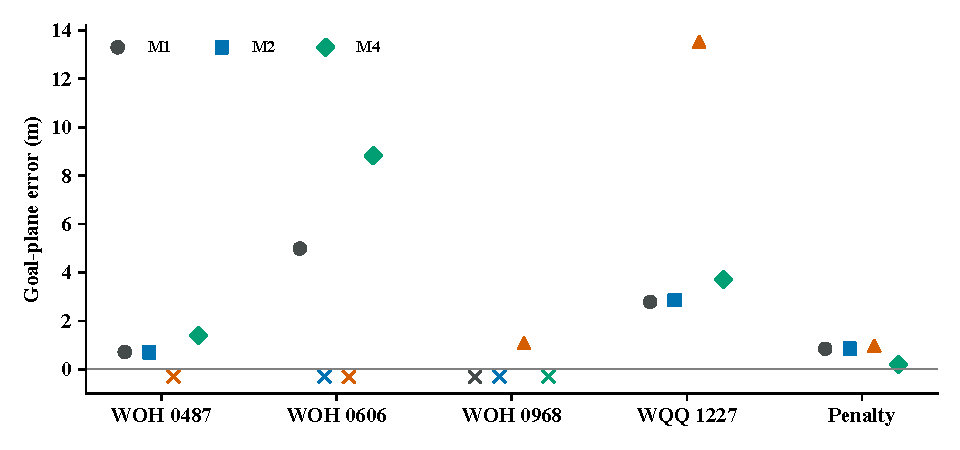
\includegraphics[width=\textwidth]{inverse_errors.pdf}
\caption{五组比赛飞行各模型的球门交点误差，每个标记对应一个事件和模型。零线下的叉号表示未给出有效球门交点，具体状态见表~\ref{tab:match-results}。}\label{fig:inverse-errors}\end{figure}
\MatchDiscussion
\begin{figure}[H]\centering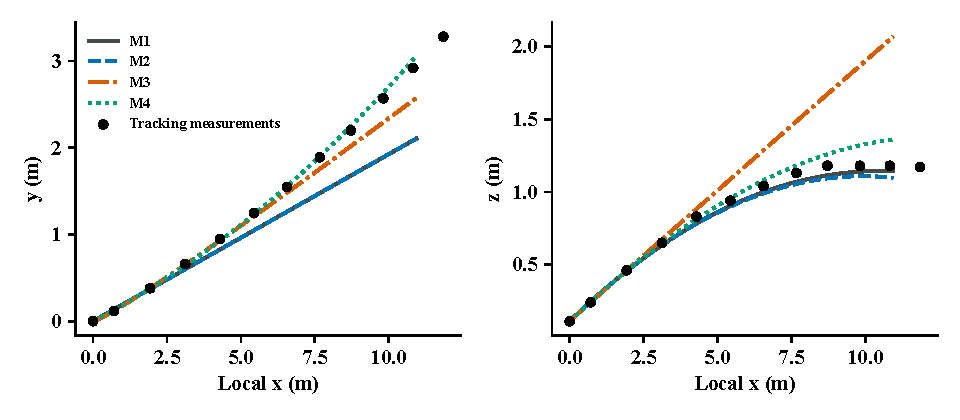
\includegraphics[width=\textwidth]{penalty_prediction.pdf}
\caption{点球记录的已收敛逆向预测及全部追踪位置。前三个位置用于反演，其余位置展示实测后续运动；各模型状态见表~\ref{tab:match-results}。}\label{fig:penalty}\end{figure}
这一对照将早期加速度与后续飞行联系起来。较大的阻力修正会造成较快的动量损失，升力修正则改变轨迹弯曲方向。因此，早期记录位移的变化会明显影响终点预测，各事件结果展示了不同模型对实际记录片段的响应。

另外，我们使用队友更正起始帧后的三例点球记录重新计算。表中数值为球门平面交点误差（m）；触地、提前终止或拟合未收敛时不列误差。
\begin{table}[H]\centering\small
\caption{更正起点后的三例点球：球门交点误差（m）}\begin{tabular}{lrrrr}\toprule
Case & M1 & M2 & M3 & M4\\\midrule
J03WMX & --- & --- & --- & 0.360\\
J03WOH & 0.684 & 0.657 & 0.374 & 0.113\\
J03WR9 & 0.550 & 0.541 & --- & ---\\
\bottomrule\end{tabular}\end{table}

\subsubsection{题目 B 算例}\label{sec:example}
题目给出的观测为
\begin{equation}
\begin{array}{c|ccc}
t\ (\mathrm{s})&x\ (\mathrm{m})&y\ (\mathrm{m})&z\ (\mathrm{m})\\\hline
0&0&0&0.11\\0.05&1.50&0.45&0.44\\0.10&2.96&0.86&0.74
\end{array}
\end{equation}
采用相同逆向流程得到表~\ref{tab:problem}，所选 M4 初始条件为
\begin{equation}
\begin{aligned}
\boldsymbol v_0&=(\ProblemVX,\ProblemVY,\ProblemVZ)\ \mathrm{m/s},\\
\boldsymbol\omega_0&=(\ProblemWX,\ProblemWY,\ProblemWZ)\ \mathrm{rad/s},\\
(C_D,\alpha)&=(\ProblemAlphaD,\ProblemAlphaL).
\end{aligned}
\end{equation}
\ProblemResultsTable
\begin{figure}[H]\centering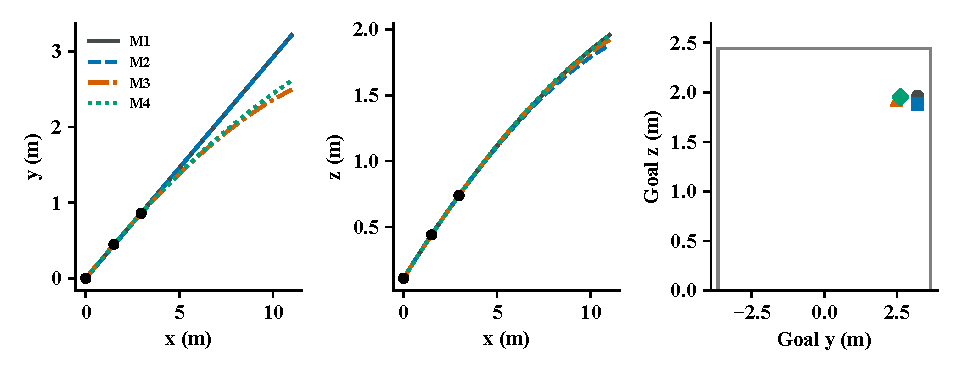
\includegraphics[width=\textwidth]{problem_prediction.pdf}
\caption{题目 B 的四类逆向预测：水平路径、竖直路径和球门平面球心位置。黑点为题目给定的早期位置。}\label{fig:problem-prediction}\end{figure}
重力和阻力保持水平速度分量之比，M1、M2 预测近似相同的水平方向。M3 延续由三点确定的恒加速度，M4 通过马格努斯力描述弯曲。M4 球心于 $\ProblemTime$ s 到达球门平面，交点为 $(\ProblemY,\ProblemZ)$ m，早期最大坐标残差为 \ProblemResidual\ m。所列自旋大小是参考设定。

\begin{figure}[H]\centering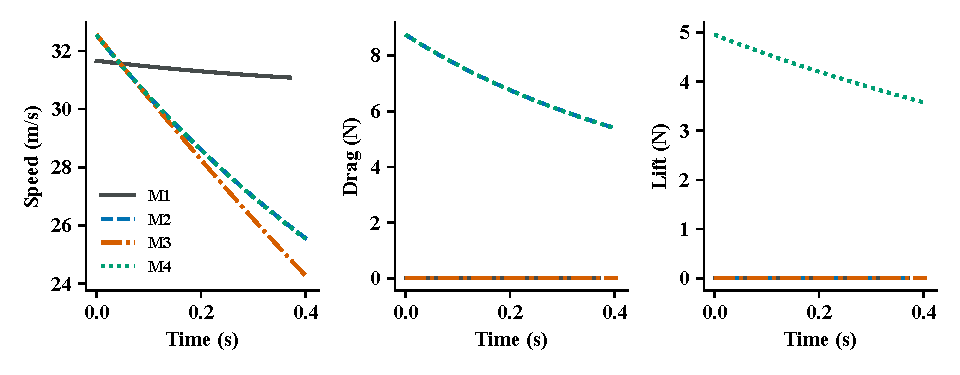
\includegraphics[width=\textwidth]{problem_dynamics.pdf}
\caption{题目 B 四类反演模型的速度与气动力大小。同一组观测在不同受力假设下给出不同后续路径。}\label{fig:problem-dynamics}\end{figure}

\subsection{案例分析：不同点球射门方式}\label{sec:kick-cases}
面对技法各异的点球，守门员只看到足球刚离脚时的几个位置，应该怎样判断球最终会飞向哪里？我们设置五类示意射门：大力、推射、侧旋弧线、上旋／后旋和挑射，并用同一套方法比较。每条轨迹先由 M4 生成，再只取 0、0.05、0.10 s 的三个位置，用 M1 和假定零自旋的 M4 预测球门交点。图中蓝色实线为模拟飞行，棕色虚线为零自旋 M4 预测，黑点是输入位置。所有数值是情景设定，不是球员统计均值\cite{alcock2012,hunteraccuracy,ravenscroft2015,carre2002}；不加入风和观测噪声。

\subsubsection*{Case 1：大力射门}
设初速度为 27 m/s、仰角 $8^\circ$，足球不自旋。球较快到达球门，本例中 M1 的球门交点误差为 0.060 m，零自旋 M4 的误差小于 0.001 m。球速快会压缩守门员的反应时间；在这组假设下，其弯曲较小，位置变化也相对容易沿早期运动方向判断。
\begin{figure}[H]\centering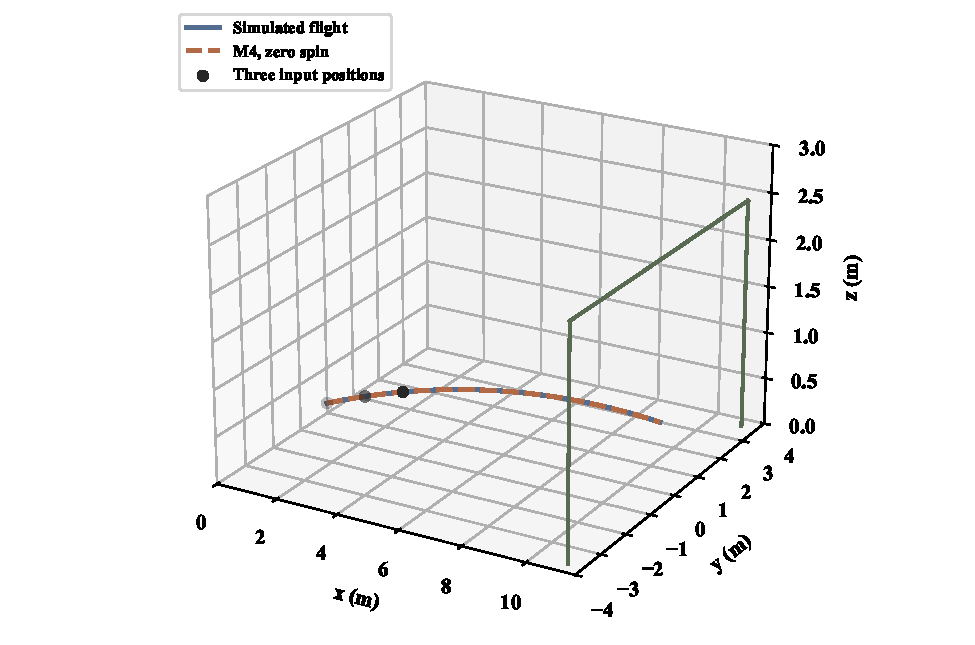
\includegraphics[width=.64\textwidth]{../results/kick_cases_linear_spin/power_3d.pdf}\caption{Case 1：大力射门的三维轨迹。}\end{figure}

\subsubsection*{Case 2：精准推射}
设初速度为 20 m/s、仰角 $11^\circ$，自旋为零。模拟球心到达球门平面的高度为 0.551 m；M1 的误差为 0.123 m，零自旋 M4 的误差小于 0.001 m。相较大力射门，球飞得较慢，守门员有更多时间观察轨迹逐步展开。
\begin{figure}[H]\centering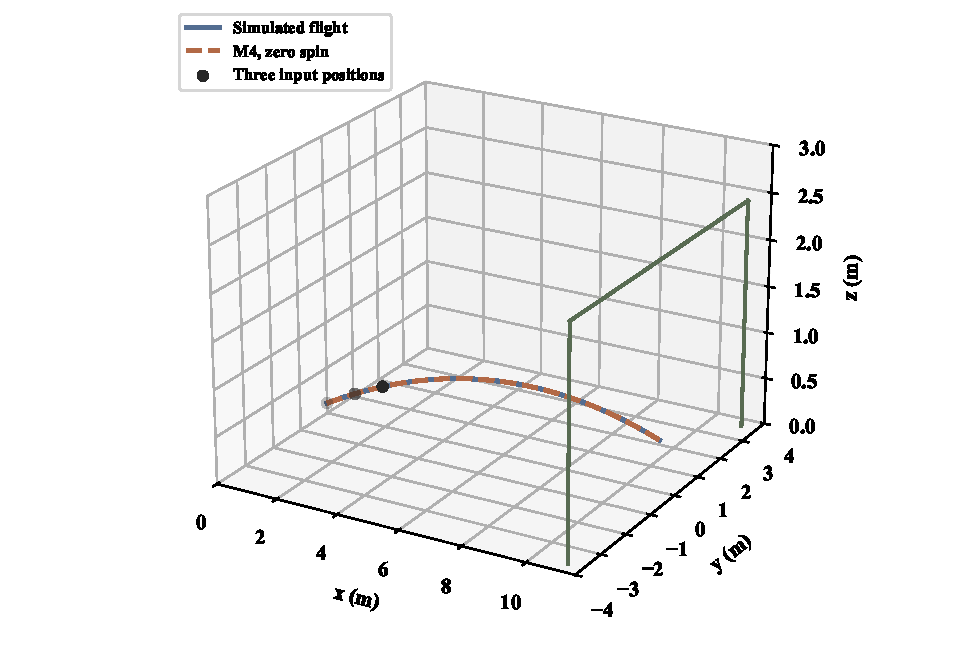
\includegraphics[width=.64\textwidth]{../results/kick_cases_linear_spin/placement_3d.pdf}\caption{Case 2：精准推射的三维轨迹。}\end{figure}

\subsubsection*{Case 3：侧旋弧线球}
设初速度为 24 m/s、仰角 $10^\circ$，初始角速度为 $(0,0,35)$ rad/s。球在飞行中向侧方弯曲，模拟交点为 $(y,z)=(0.841,0.877)$ m；如果预测时忽略自旋，M4 的交点误差为 0.688 m。守门员看到的早期横向运动可能同时包含初始方向和旋转效应，因此需要给后续弯曲留出判断余地。
\begin{figure}[H]\centering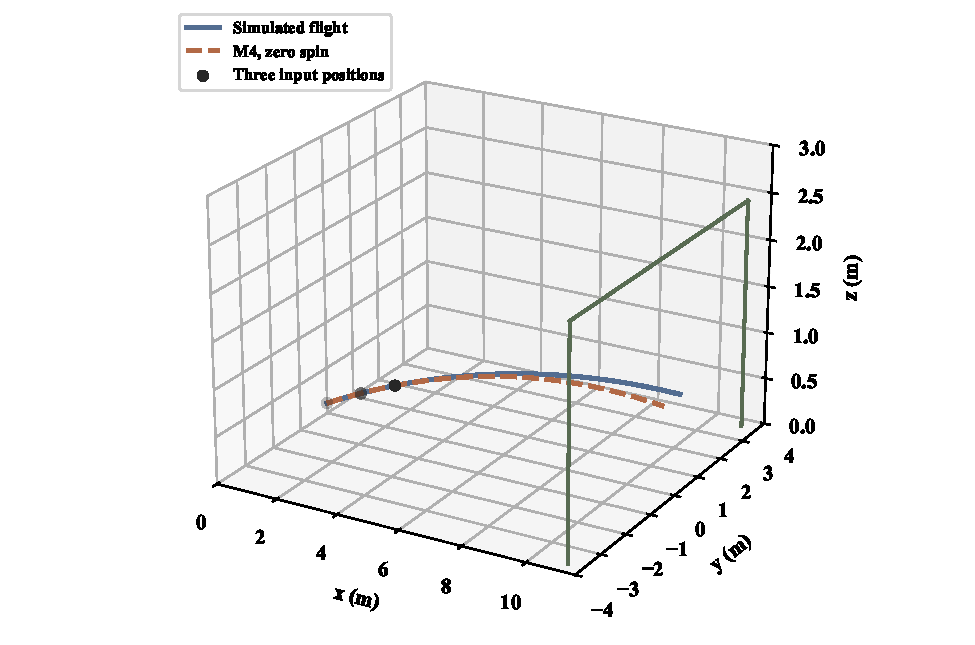
\includegraphics[width=.64\textwidth]{../results/kick_cases_linear_spin/curved_3d.pdf}\caption{Case 3：侧旋弧线球的三维轨迹。}\end{figure}

\subsubsection*{Case 4：上旋与后旋}
两种情况的初速度均为 24 m/s。上旋取仰角 $12^\circ$、角速度 $(0,35,0)$ rad/s；后旋取仰角 $10^\circ$、角速度 $(0,-35,0)$ rad/s。两者的模拟球门高度分别为 0.426 m 和 1.723 m；若预测时假定零自旋，M4 的误差分别为 0.682 m 和 0.692 m。旋转方向改变了竖直弯曲，守门员除了判断左右位置，还需要关注球的高度变化。
\begin{figure}[H]\centering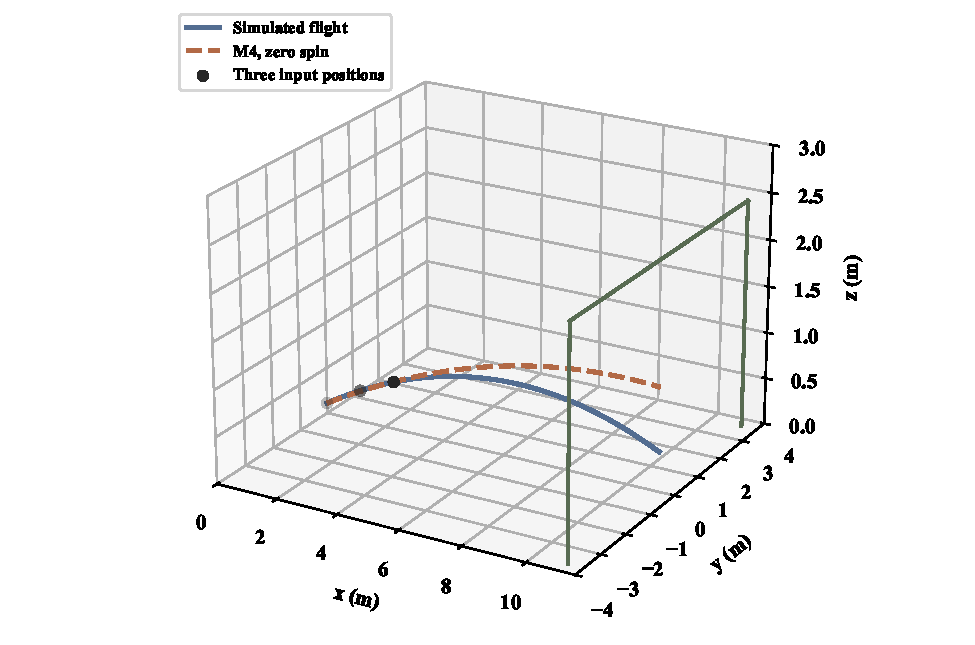
\includegraphics[width=.48\textwidth]{../results/kick_cases_linear_spin/topspin_3d.pdf}\hfill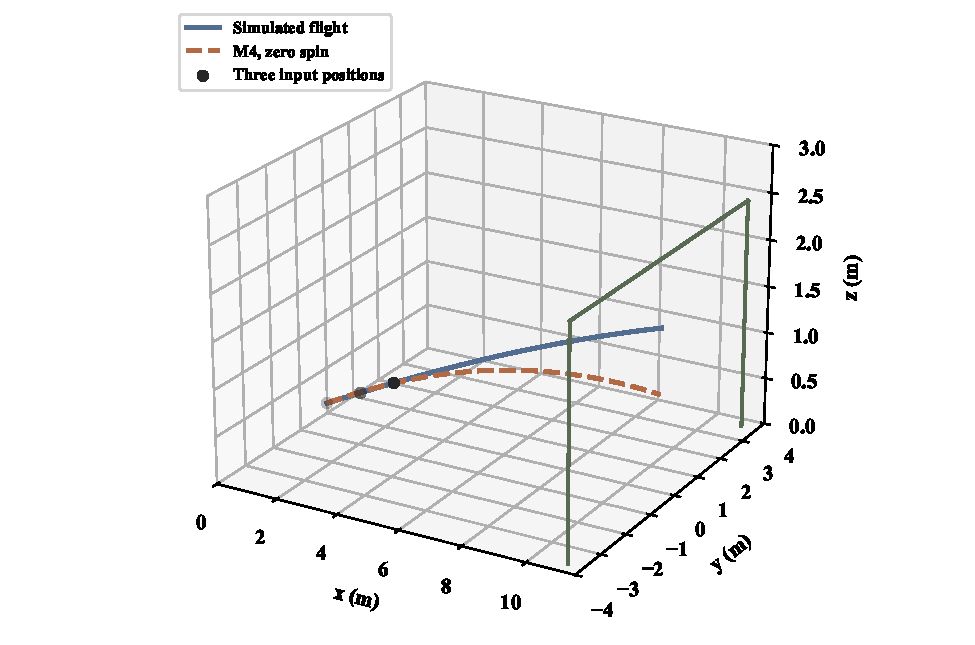
\includegraphics[width=.48\textwidth]{../results/kick_cases_linear_spin/backspin_3d.pdf}\caption{Case 4：上旋（左）与后旋（右）。}\end{figure}

\subsubsection*{Case 5：挑射}
设初速度为 14 m/s、仰角 $20^\circ$，并赋予 $(0,-15,0)$ rad/s 的后旋。相对较低的速度和较大的仰角使轨迹先升后降，模拟球门高度为 0.941 m；M1 与零自旋 M4 的误差分别为 0.250 m 和 0.555 m。面对挑射，守门员需要判断球经过上升阶段后的下落位置。
\begin{figure}[H]\centering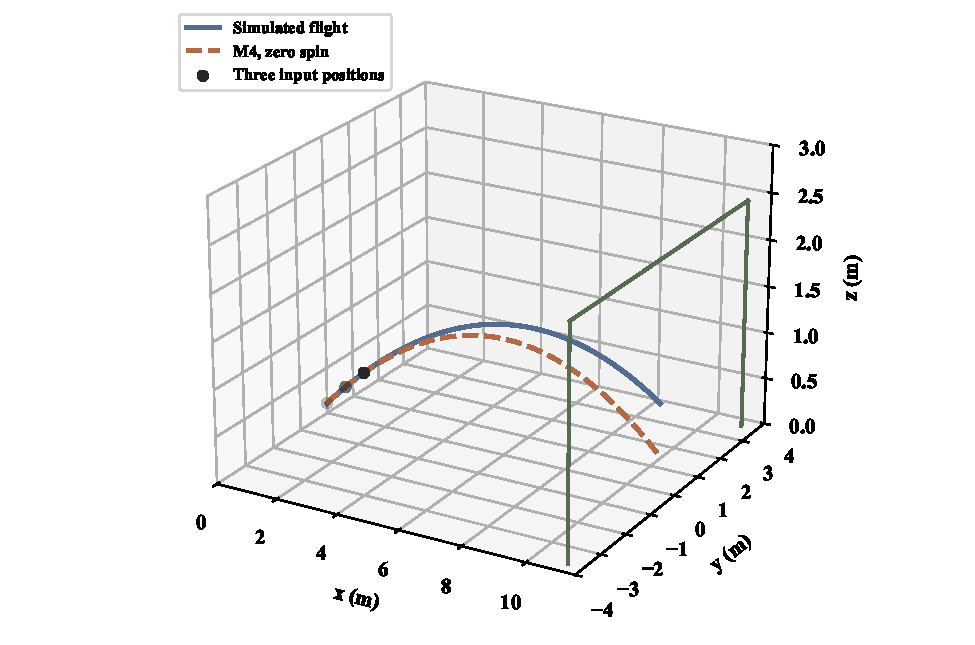
\includegraphics[width=.64\textwidth]{../results/kick_cases_linear_spin/chip_3d.pdf}\caption{Case 5：挑射的三维轨迹。}\end{figure}

\paragraph{案例汇总。} 表~\ref{tab:kick-cases} 汇总六条轨迹。已知自旋的 M4 是条件对照：它额外使用仿真真值中的自旋；生成和预测采用同一方程，因此误差接近零。这里每类只选一条合成轨迹，用于展示自旋可能造成的影响；真实比赛射门的独立对照仍见第~\ref{sec:real-validation} 节。案例使用固定 $C_D$ 和 $\alpha$。
\begin{table}[H]\centering\small\caption{六条示意射门的三点预测汇总；误差为球门平面距离}\label{tab:kick-cases}
\begin{tabular}{lrrrrrr}\toprule
案例 & $v_0$ & 仰角 & 自旋 $(\omega_y,\omega_z)$ & M1 & M4 零自旋 & M4 已知自旋\\
 & (m/s) & (度) & (rad/s) & (m) & (m) & (m)\\\midrule
大力射门 & 27 & 8 & $(0,0)$ & 0.060 & $<0.001$ & $<0.001$\\
精准推射 & 20 & 11 & $(0,0)$ & 0.123 & $<0.001$ & $<0.001$\\
侧旋弧线 & 24 & 10 & $(0,35)$ & 0.693 & 0.688 & $<0.001$\\
上旋 & 24 & 12 & $(35,0)$ & 0.764 & 0.682 & $<0.001$\\
后旋 & 24 & 10 & $(-35,0)$ & 0.610 & 0.692 & $<0.001$\\
挑射 & 14 & 20 & $(-15,0)$ & 0.250 & 0.555 & $<0.001$\\\bottomrule
\end{tabular}\end{table}

\section{灵敏性分析}\label{sec:sensitivity}
\textit{待完成。}

\section{其他因素讨论}\label{sec:other}
本节讨论表面几何、自旋演化和环境来流的影响。
\subsection{足球表面的非对称几何}\label{sec:surface}
Paudel 和 Yan\cite{paudel} 利用真实足球几何进行全程流动模拟，并与光滑球比较。在初速度 10、15、20 m/s，自旋 31.5、63、94.5 rad/s 的工况下，接缝和表面结构会改变流动分离、尾流演化及马格努斯力。九组对照中光滑球的横向弯曲均更强，较高速度和转速下竖直飞行时间的差异也更明显。

\begin{figure}[H]\centering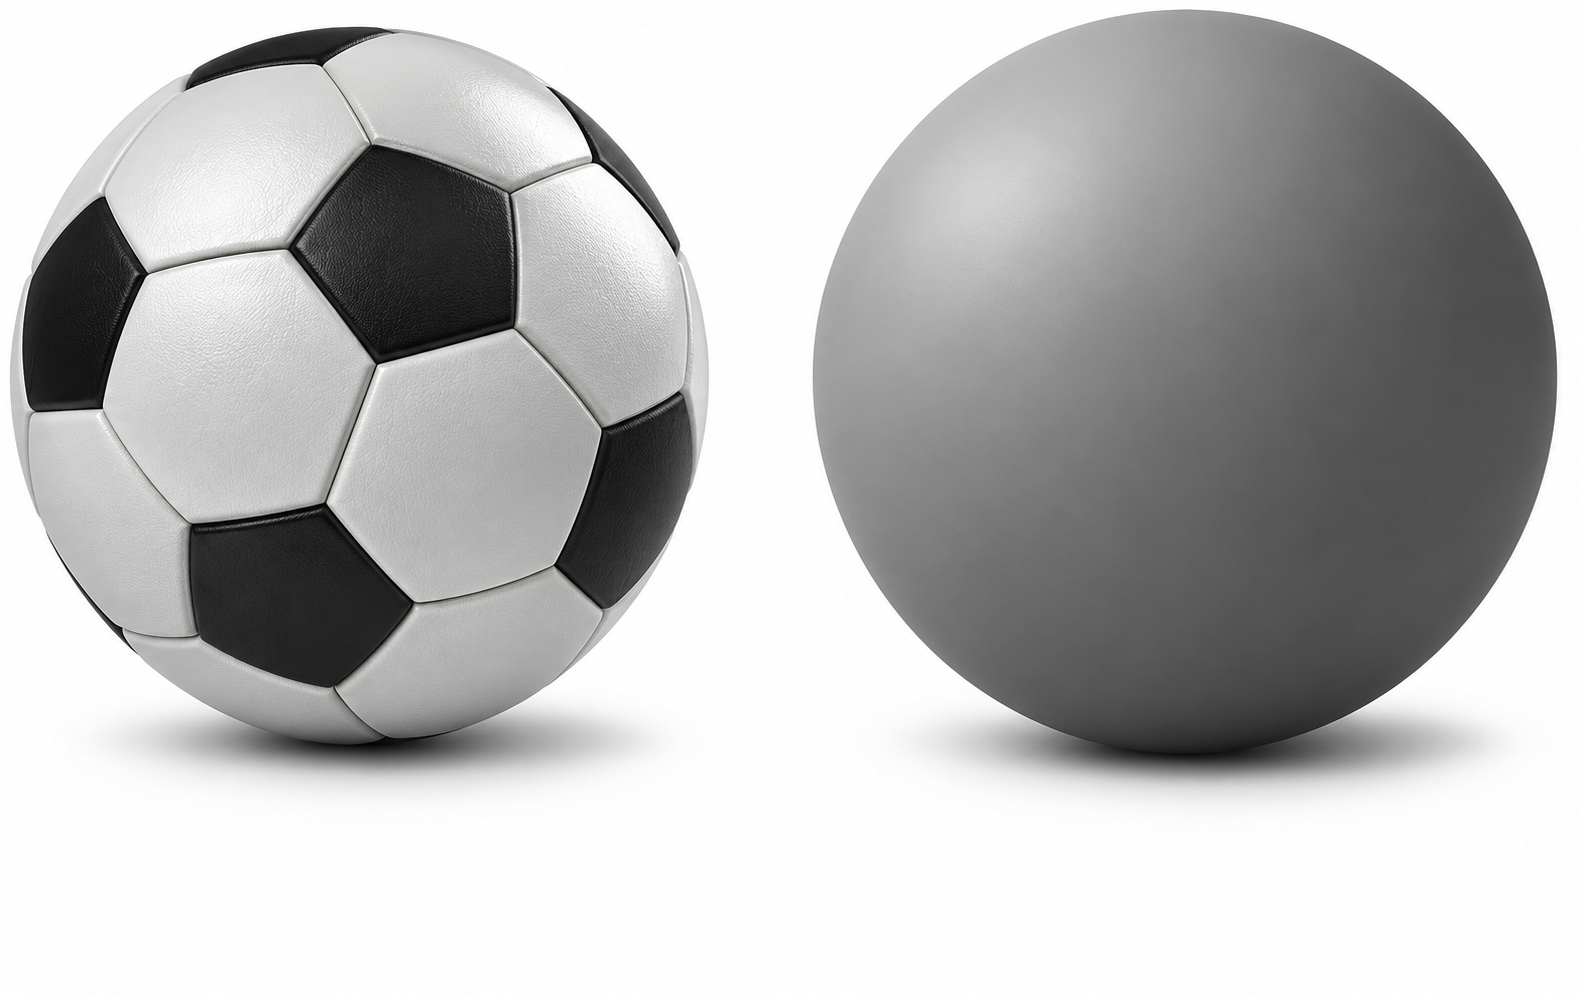
\includegraphics[width=.60\textwidth]{surface_comparison.png}
\caption{有面板接缝的足球与光滑球体示意图，参考 Paudel 和 Yan 的比较\cite{paudel}；原研究中两球直径均为 0.22 m、质量均为 0.436 kg。图中面板形状仅作示意。}\label{fig:surface-geometry}\end{figure}

Alam 等\cite{alam2012} 的风洞实验表明，不同足球表面结构会影响阻力系数。

\begin{figure}[H]\centering
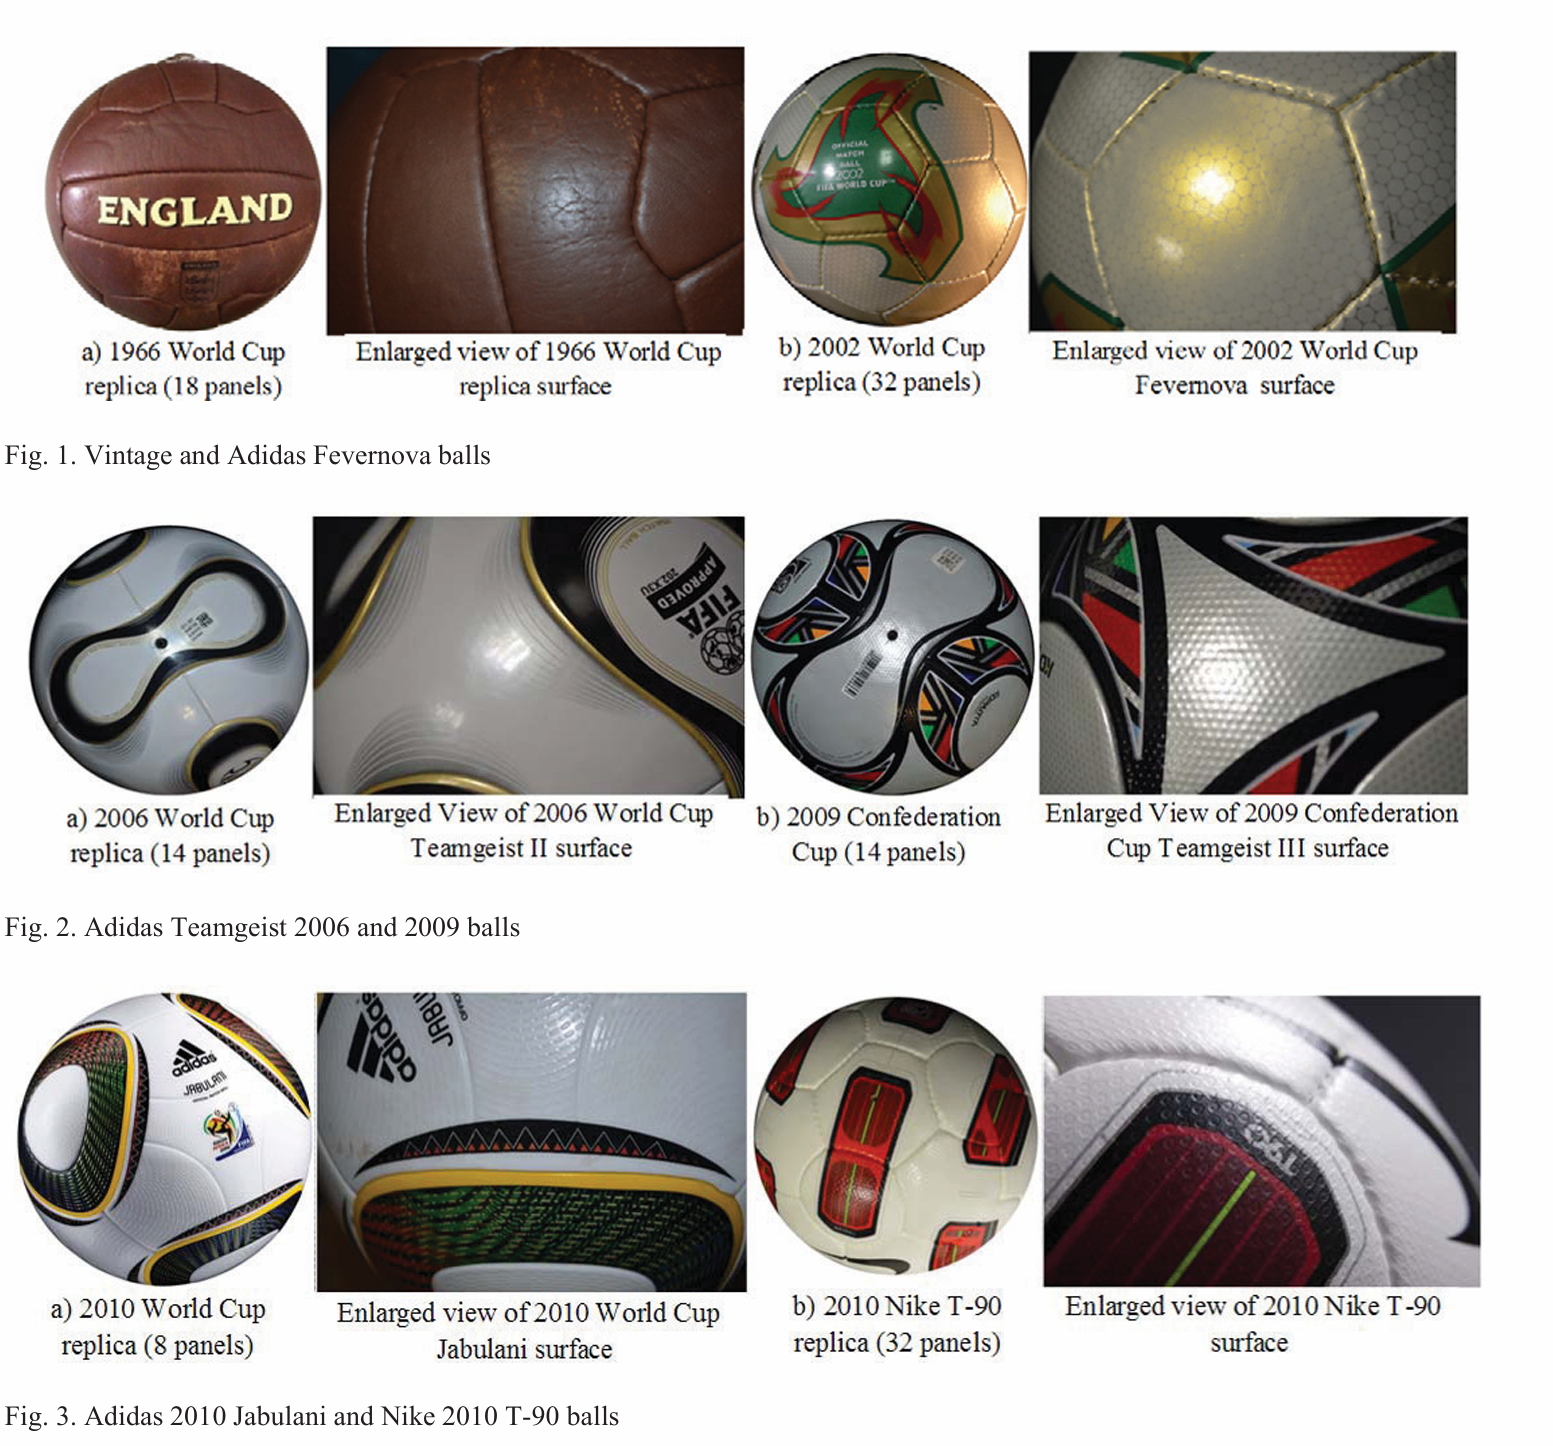
\includegraphics[width=.86\textwidth]{alam_ball_surfaces.png}
\caption{六种足球及其表面细节，原图为 Alam 等\cite{alam2012} 的图 1--3。}\label{fig:alam-surfaces}\end{figure}

\begin{figure}[H]\centering
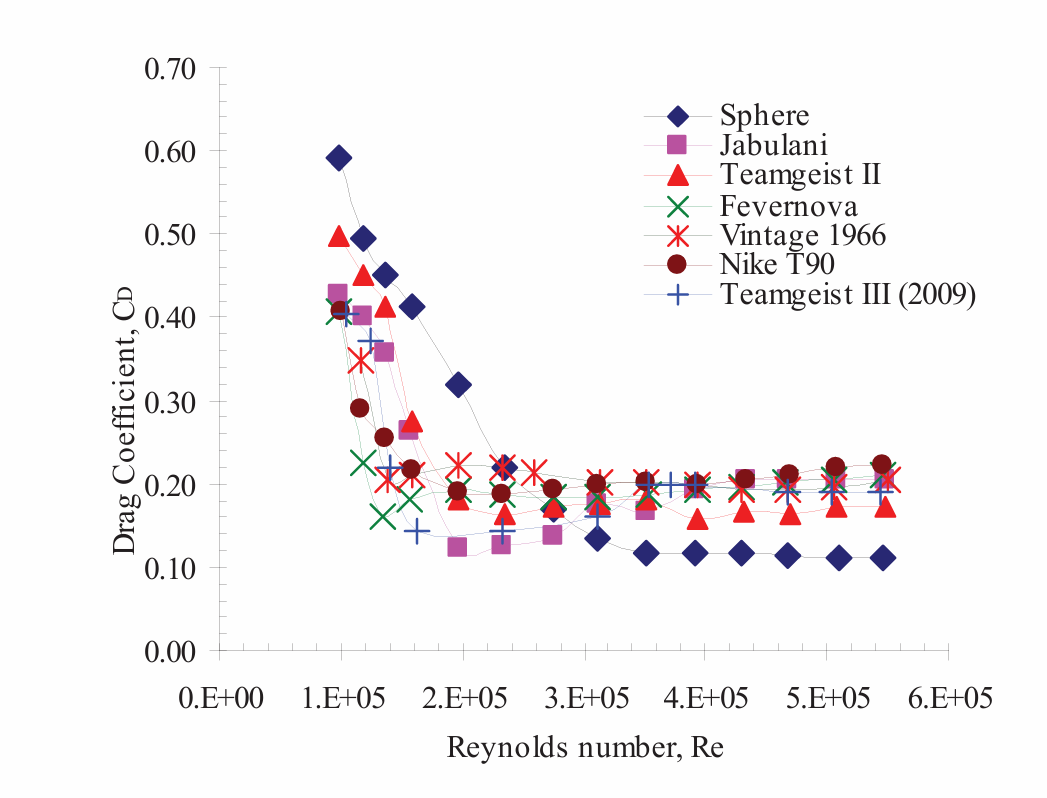
\includegraphics[width=.76\textwidth]{alam_drag_comparison.png}
\caption{不同足球和光滑球的阻力系数随雷诺数变化，来源：Alam 等\cite{alam2012}，图 5。}\label{fig:alam-drag}\end{figure}

本文的球形几何描述质心运动与迎风面积，气动力系数来自足球实验，因此表面的平均作用已进入 $C_D$、$C_L$。当侧向力细节更为重要时，可进一步描述面板朝向与非对称尾流波动。这些文献结果说明，在球形轨迹模型中保留足球专用气动系数具有物理依据。

\subsection{足球旋转与气动阻尼}\label{sec:rotation}
空气阻力矩会使自旋减弱\cite{grad2026,mujoco381}；本节主模型取恒定自旋。线性自旋升力公式可以用于后续比较不同自旋大小和阻尼作用。

\subsection{风速与气动力估算}\label{sec:wind}
风通过 $\boldsymbol u=\boldsymbol v-\boldsymbol v_{\rm wind}$ 改变相对来流\cite{maponi}。暂保持气动系数不变，沿飞行方向大小为 $w$ 的风使动压尺度变为
\begin{equation}
\frac{q_{\rm head}}{q_0}=(1+w/v)^2,\qquad
\frac{q_{\rm tail}}{q_0}=(1-w/v)^2,\qquad
\frac{q_{\rm cross}}{q_0}=1+(w/v)^2.
\end{equation}
横风还使来流转过 $\arctan(w/v)$，从而改变气动力方向。表~\ref{tab:wind} 在反演初速度下给出上述粗略估算，列示风速作为比较工况。
\WindResultsTable
将逆风动压增幅限制在 5\% 时，有 $w/v\leq\sqrt{1.05}-1$，对应本算例的 $w\leq\WindThreshold$ m/s。静止空气近似更适合室内或弱风飞行；风速较大时应通过相对速度纳入计算。

\section{小结}
模型将足球飞行与重力、浮力、阻力和马格努斯升力联系起来；本文所列数值采用未计浮力的三力基准计算。M4 使用固定阻力系数与线性自旋升力，以减少待拟合参数。

受控无旋转算例说明，阻力对射程预测十分重要；M4 预测 \ForwardMFourRange\ m，文献实测为 21.9 m。旋转轨迹片段展示了上旋造成的向下弯曲，以及同一系数关系在不同算例中的表现差异。比赛记录对照则说明早期位移和拟合修正系数如何影响后续预测。

对于题目 B，M4 的球门交点为 $(y,z)=(\ProblemY,\ProblemZ)$ m。马格努斯力解释了其与仅含重力、阻力模型之间明显的水平差别。风的估算给出了静止空气近似对应的弱风条件，灵敏性分析结论将在第五章完成后补充。

\section{模型评价}
\subsection{物理解释与计算应用}
模型层级使各力的作用清晰可见，同一套动力学支持正向求解、早期位置反演和终点预测。气动力修正系数直接联系实测轨迹差异，各实验与数值输入均保留相应来源。
\subsection{预测表现与改进方向}
风洞系数、受控发射和比赛飞行分别考察系数趋势、曲率与射程、以及依据早期位置进行预测的表现。逐事件误差展示了经验足球系数与早期轨迹对后续运动的描述情况。球型专用气动测量、直接自旋测量和同步高频位置记录有助于改善预测，具体应用还可纳入表面朝向、旋转阻尼与风。
\addcontentsline{toc}{section}{参考文献}
\begin{thebibliography}{99}
\raggedright
\bibitem{kamp2018} J. van der Kamp, M. Dicks, J. A. Navia and B. No\"el, ``Goalkeeping in the soccer penalty kick,'' \emph{German Journal of Exercise and Sport Research}, 48, 169--175, 2018. \url{https://doi.org/10.1007/s12662-018-0506-3}.
\bibitem{hunter2018} A. H. Hunter, S. C. Murphy, M. J. Angilletta Jr. and R. S. Wilson, ``Anticipating the direction of soccer penalty shots depends on the speed and technique of the kick,'' \emph{Sports}, 6, 73, 2018. \url{https://doi.org/10.3390/sports6030073}.
\bibitem{griffiths2005} I. Griffiths, C. Evans and N. Griffiths, ``Tracking the flight of a spinning football in three dimensions,'' \emph{Measurement Science and Technology}, 16, 2056--2065, 2005. \url{https://doi.org/10.1088/0957-0233/16/10/022}.
\bibitem{goff2017} J. E. Goff, J. Kelley, C. M. Hobson, K. Seo, T. Asai and S. B. Choppin, ``Creating drag and lift curves from soccer trajectories,'' \emph{European Journal of Physics}, 38, 044003, 2017. \url{https://doi.org/10.1088/1361-6404/aa6fcd}.
\bibitem{bray} K. Bray and D. G. Kerwin, ``Modelling the flight of a soccer ball in a direct free kick,'' \emph{Journal of Sports Sciences}, 21, 75--85, 2003. \url{https://doi.org/10.1080/0264041031000070994}.
\bibitem{alcock2012} A. Alcock, W. Gilleard, N. A. T. Brown, J. Baker and A. Hunter, ``Initial ball flight characteristics of curve and instep kicks in elite women's football,'' \emph{Journal of Applied Biomechanics}, 28, 70--77, 2012. \url{https://doi.org/10.1123/jab.28.1.70}.
\bibitem{ravenscroft2015} J. C. Ravenscroft and N. P. Linthorne, ``Effect of the location of the foot impact point on ball velocity in a soccer penalty kick,'' \emph{33 International Conference of Biomechanics in Sports}, 2015. \url{https://ojs.ub.uni-konstanz.de/cpa/article/view/6595}.
\bibitem{carre2002} M. J. Carr\'e, T. Asai, T. Akatsuka and S. J. Haake, ``The curve kick of a football II: flight through the air,'' \emph{Sports Engineering}, 5, 193--200, 2002. \url{https://doi.org/10.1046/j.1460-2687.2002.00109.x}.
\bibitem{hunteraccuracy} A. H. Hunter, M. J. Angilletta Jr., T. Pavlic, G. Lichtwark and R. S. Wilson, ``Modeling the two-dimensional accuracy of soccer kicks,'' \emph{Journal of Biomechanics}, 72, 159--166, 2018. \url{https://doi.org/10.1016/j.jbiomech.2018.03.003}.
\bibitem{bassek} M. Bassek, R. Rein, H. Weber and D. Memmert, ``An integrated dataset of spatiotemporal and event data in elite soccer,'' \emph{Scientific Data}, 12, 195, 2025. \url{https://doi.org/10.1038/s41597-025-04505-y}.
\bibitem{dataset} DFL, ``Sportec Open DFL Dataset,'' CC BY 4.0. 数据镜像： \url{https://huggingface.co/datasets/pysport/idsse-data}.
\bibitem{maponi} P. Maponi and R. Piombin, ``A computational framework to predict the soccer ball trajectory,'' \emph{Journal of Applied Mathematics}, 2025, 7425581. \url{https://doi.org/10.1155/jama/7425581}.
\bibitem{alam2012} F. Alam, H. Chowdhury, M. Stemmer, Z. Wang and J. Yang, ``Effects of surface structure on soccer ball aerodynamics,'' \emph{Procedia Engineering}, 34, 146--151, 2012. \url{https://doi.org/10.1016/j.proeng.2012.04.026}.
\bibitem{paudel} S. Paudel and J. Yan, ``High-fidelity simulations of full-flight soccer ball aerodynamics using a monolithic overset approach,'' \emph{Computational Mechanics}, 77, 1245--1265, 2026. \url{https://doi.org/10.1007/s00466-025-02705-2}.
\bibitem{myers} T. G. Myers and S. L. Mitchell, ``A mathematical analysis of the motion of an in-flight soccer ball,'' \emph{Sports Engineering}, 16, 29--41, 2013. \url{https://doi.org/10.1007/s12283-012-0105-8}.
\bibitem{asai2007} T. Asai, K. Seo, O. Kobayashi and R. Sakashita, ``Fundamental aerodynamics of the soccer ball,'' \emph{Sports Engineering}, 10, 101--110, 2007. \url{https://doi.org/10.1007/BF02844207}.
\bibitem{kiratidis2018} A. L. Kiratidis and D. B. Leinweber, ``An aerodynamic analysis of recent FIFA World Cup balls,'' \emph{European Journal of Physics}, 39, 034001, 2018. \url{https://doi.org/10.1088/1361-6404/aaa888}. 公式及参数： \url{https://arxiv.org/abs/1710.02784v2}.
\bibitem{grad2026} \L{}. Grad, K. M. Czajkowski and A. Varashylau, ``Physics-Based 3D Ball Trajectory Reconstruction from Monocular Soccer Video: A Multi-Model Benchmark,'' \emph{Proceedings of the IEEE/CVF Conference on Computer Vision and Pattern Recognition Workshops}, 9940--9948, 2026. \href{https://openaccess.thecvf.com/content/CVPR2026W/CVsports/supplemental/Grad_Physics-Based_3D_Ball_CVPRW_2026_supplemental.pdf}{补充材料}, 第 8.4 节.
\bibitem{mujoco381} MuJoCo developers, MuJoCo 3.8.1, ellipsoid fluid model, \texttt{mj\_viscousForces} in \texttt{src/engine/engine\_passive.c}. \href{https://github.com/google-deepmind/mujoco/blob/3.8.1/src/engine/engine_passive.c}{3.8.1 版源代码}; 默认旋转阻力： \href{https://mujoco.readthedocs.io/en/stable/XMLreference.html#body-geom-fluidcoef}{XML 参考，geom/fluidcoef}. 访问日期：2026 年 11 月 8 日。
\bibitem{goff2009} J. E. Goff and M. J. Carr\'e, ``Trajectory analysis of a soccer ball,'' \emph{American Journal of Physics}, 77, 1020--1027, 2009. \url{https://doi.org/10.1119/1.3197187}.
\end{thebibliography}

\newpage\addcontentsline{toc}{section}{复现代码}
\section*{复现代码}
随附项目包含固定输入、矢量标记提取、四模型计算、结果表及制图脚本。以下节选展示统一状态方程和受力计算。逆向求解按第~\ref{sec:inverse} 节的所述多初值方法调用同一状态导数。计算与制图分别执行，可直接利用保存结果更新图表。
\lstinputlisting[language=Python,firstline=177,lastline=181]{../src/football/physics/model.py}
\lstinputlisting[language=Python,firstline=217,lastline=237]{../src/football/physics/model.py}
\end{document}
